\documentclass[stu, a4paper, 12pt, floatsintext]{apa7}

% Title Page Stuff
\title{A Comparative Analysis of Aireon’s Space-based ADS-B Technology and Other Alternatives for Air Traffic Management}
\shorttitle{Space-Based ADS-B Analysis}
\leftheader{25/04/25}
\authorsnames{Philip Beswick @00662943}
\authorsaffiliations{The University of Salford}
\course{Aircraft Engineering with Pilot Studies}
\professor{Miss Frances Wolff, Dr Viktoriia Myroniuk}
\duedate{25/04/25}
\keywords{}
\authornote{}
\abstract{}

% Packages Required
\usepackage{csquotes}
\usepackage[english]{babel}
\usepackage[T1]{fontenc}
\usepackage{mathptmx}
\usepackage{multirow}
\usepackage{graphicx}
\usepackage{booktabs}
\usepackage[style=apa,sortcites=true,sorting=nyt,backend=biber]{biblatex}
\usepackage{pgf-pie}
\usepackage{pgfplots}
\usepackage{paracol}
\usepackage{amsmath}
\usepackage{tocloft}
\usepackage{float}
\usepackage{listings}
\usepackage{gensymb}

\addbibresource{bibliography.bib}

\pgfplotsset{compat=1.18}

% Counts chapters numerically
\setcounter{tocdepth}{5}
\setcounter{secnumdepth}{5}

% Counts equations, figures and tables sequentially depending on the chapter
\numberwithin{figure}{section}
\numberwithin{table}{section}
\numberwithin{equation}{section}

\newcommand{\listequationsname}{\Large List of Equations}
\newlistof{myequations}{equ}{\listequationsname}
\newcommand{\myequations}[1]{%
\addcontentsline{equ}{myequations}{\protect\numberline{\theequation}#1}\par}
\setlength{\cftmyequationsnumwidth}{2.5em}% Width of equation number in List of Equations

% Makes sure LaTeX knows where we are :D
\DeclareLanguageMapping{british}{british-apa}

\begin{document}

\maketitle{} % Generates the title page

\tableofcontents
\newpage

\addcontentsline{toc}{subsection}{List of Figures}
\listoffigures
\addcontentsline{toc}{subsection}{List of Tables}
\listoftables
\addcontentsline{toc}{subsection}{List of Equations}
\listofmyequations

\newpage
\section{Introduction}
Space-based ADS-B has the potential to be the next generation in aircraft surveillance and aircraft tracking due to its global coverage, which is especially important for remote areas, such as the North Atlantic Ocean, where it was not previously possible to track aircraft on traditional RADAR. From 2017 to 2023, SpaceX launched 66 satellites, which housed the Space-based ADS-B technology developed by Aireon, and since the technology has been trialled by NATS and Nav Canada over the North Atlantic Ocean. 

Traditionally, aircraft are surveilled in all phases of flight, from before they power up their engines on the apron to when they power down at their destination, aircraft are constantly monitored by and communicate with Air Traffic Controllers. Aircraft are monitored by Primary and Secondary RADAR as well as ADS-B systems. Usually, a combination of these different approaches is used to get the most accurate information about the state of an aircraft. ADS-B has, however, become increasingly popular and more widely used in contrast with primary and secondary radar for aircraft surveillance. This is because ADS-B technology is comparatively much cheaper than RADARs while also providing additional capabilities, such as Air-to-Air surveillance, that RADAR does not (\cite{AvionixTech}). Yet, both ADS-B and RADAR have the same limitation - they require a line-of-sight between aircraft and ground stations to function.

In some parts of the world, the installation of a ground station is simply not possible. This could be due to an extreme financial cost that would be incurred in very remote areas, or due to physical impossibilities, such as over Oceans. Therefore, over large portions of the planet, it is not possible to provide aircraft tracking or surveillance services. This is especially true over the North Atlantic Ocean.  

In 2012, approximately 460000 flights crossed the North Atlantic Ocean (\cite{SKYbrary}), with this number rising to over 580000 in 2023 (\cite{ForeFlight}) making the airspace some of the busiest in the world. This means that around 1500 aircraft make the trans-Atlantic crossing every single day. Keeping aircraft safe while making this crossing is made difficult by the lack of tracking or surveillance services that were previously mentioned. So, the Organised Track System was developed. 
\subsection{The Organised Track System}
The Organised Track System (OTS) was designed to ensure aircraft remain safely separated when flying across the North Atlantic Ocean. Each day, Nav Canada and NATS jointly publish a list of directional “tracks” across the North Atlantic airspace, with each track following a great circle (\cite{OTS}). Figure 1.1 below, shows the Eastbound and Westbound tracks that were in use on April 7th 2025. 

\begin{figure}[H]
    \caption{An image taken from the RADAR software showing the North Atlantic tracks that were used on April 7th 2025. NAT A and NAT W are labelled.}
    \label{fig:1.1}
    \centering
    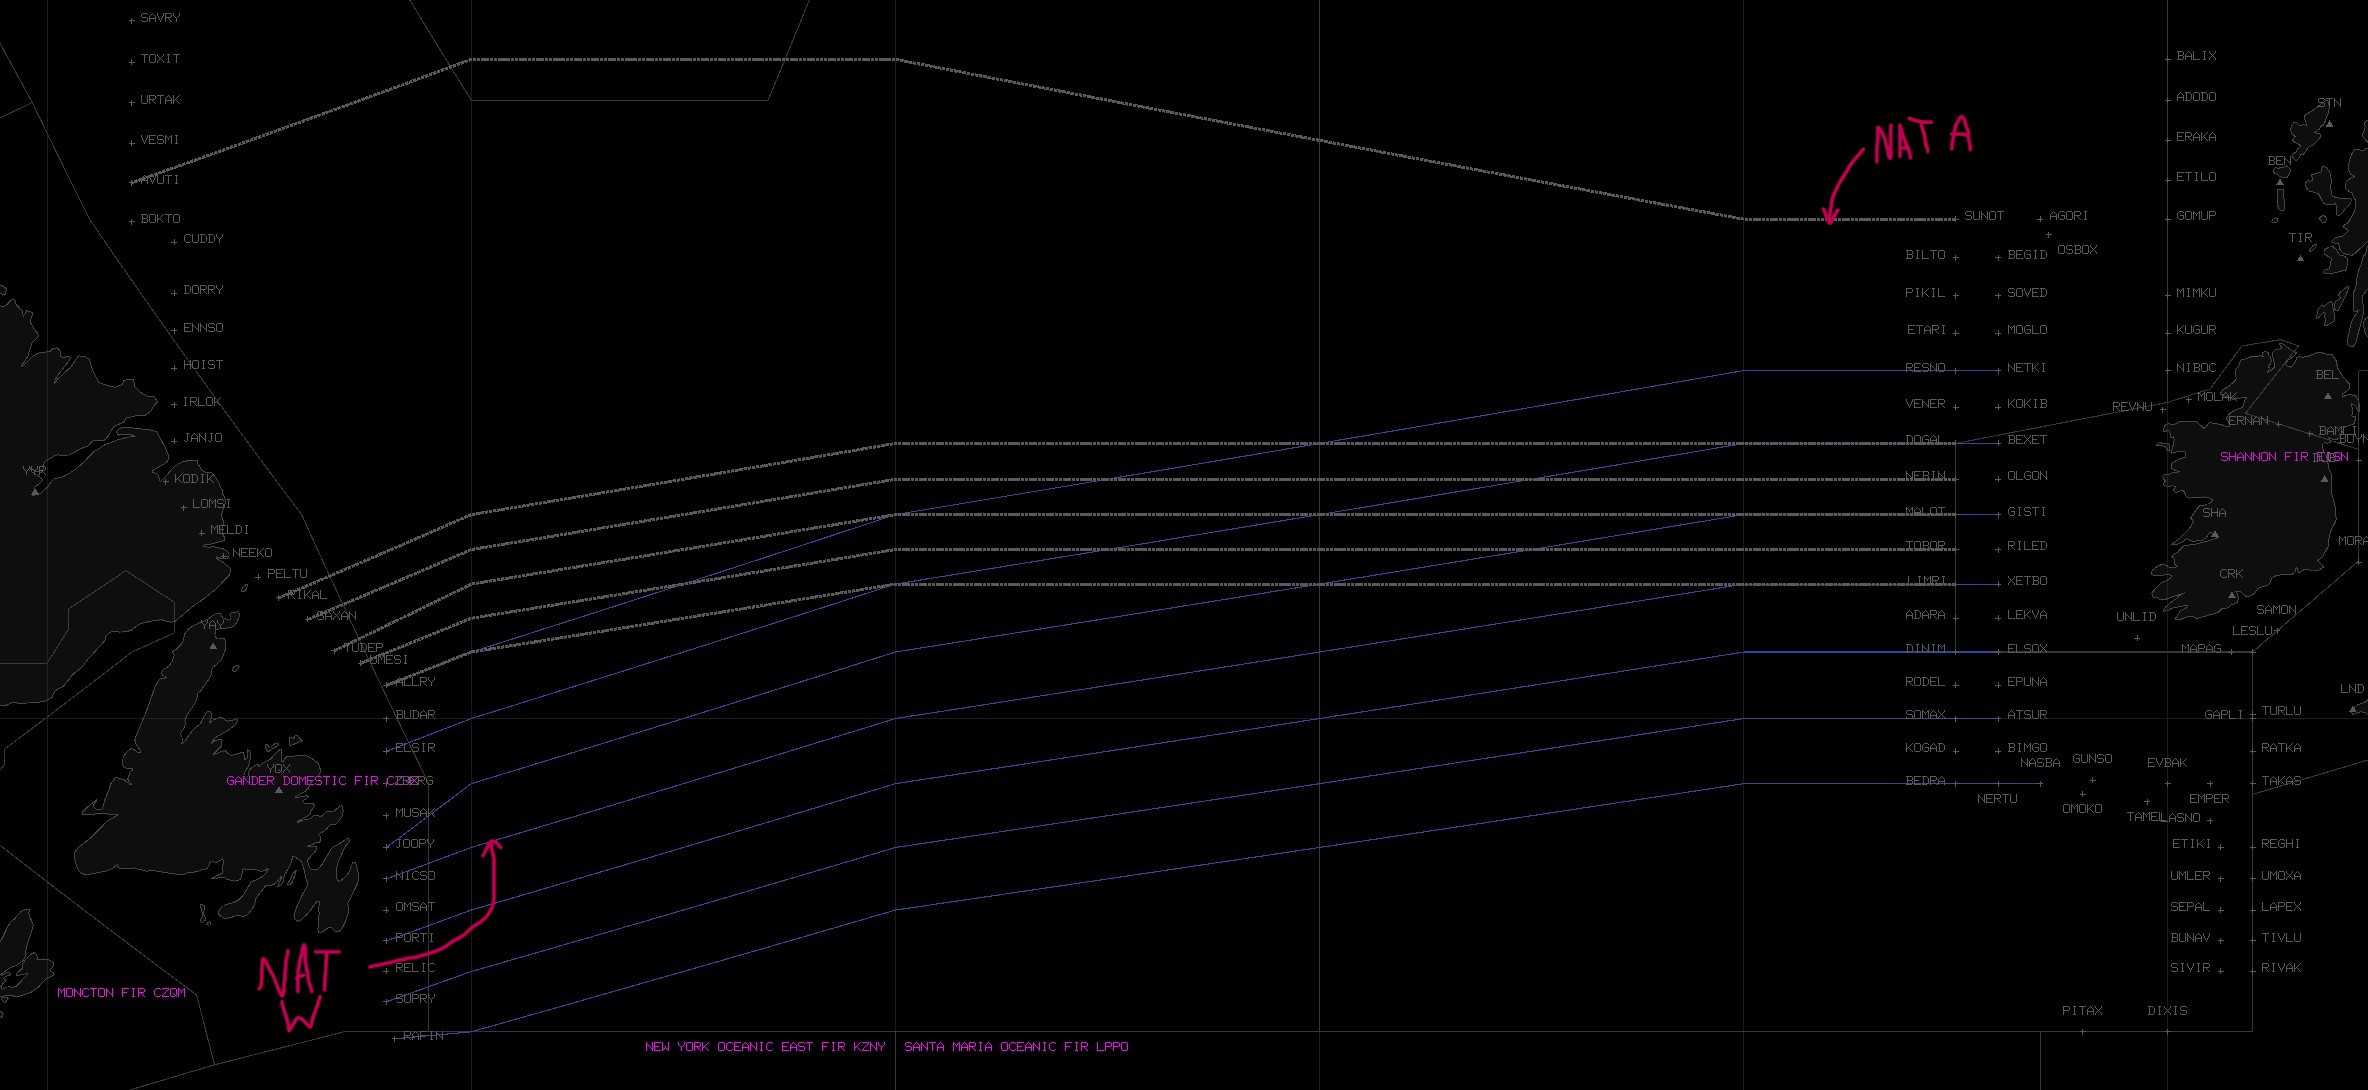
\includegraphics[width=1.1\textwidth]{pictures/Figure 1.1.jpg}    
\end{figure}

As alluded to previously, these tracks are directional, this means that each track has traffic operating in only one direction. For example, in Figure 1.1 above, North Atlantic Track (NAT) A carries traffic moving westbound, whereas NAT W carries traffic moving eastbound. In order for an aircraft to make the crossing over the Atlantic, they must fly on one of the designated tracks, starting and ending at that track's respective entry and exit points. To further aid in the smooth running, at any given time, tracks are only ever in use in one direction. For 12 hours each day only the eastbound tracks are in use and for the other 12 hours westbound tracks are in use. For anyone who has ever made a trans-atlantic flight, this is why flights from Europe to the United States of America tend to leave Europe in the early morning, but when making the return journey, they leave the United States in the late evening. 

So, the existence of tracks means at any given point in time, Air Traffic Controllers are aware of which track an aircraft is on and by extension, which way they are going. However, there is still no way of monitoring their progress once they enter the track. Therefore, strict separation requirements are enforced. These are (\cite{SKYbrary}):
\begin{enumerate}
    \item One Degree of latitude, approximately 60 NM, for aircraft on the same track,
    \item 1000ft of vertical separation.
\end{enumerate}

This is monitored by voice communications over HF Radio. Every 15 minutes, aircraft provide a position report, stating their current coordinates in latitude and longitude, speed, heading and altitude, following where they expect to be in 15 minutes' time. Using this, Air Traffic Controllers are able to build up a picture of all the aircraft along a track, and can ensure there is enough vertical and horizontal separation between all aircraft at any given point in time.

Additionally, Air Traffic Controllers are able to plan for aircraft operating at different speeds, so faster moving aircraft won’t be held up by other aircraft flying much slower.

The main limitation of the OTS is the tracks themselves. On any given day, only a small number of routes are available across the Atlantic. The routes are designed to be the most optimal for all traffic, generally, when accounting for the wind direction and speed. Unfortunately, these tracks can never be perfect for all operators flying across the Atlantic each day. Often, aircraft have to fly out of their way to reach a NAT entry point, or are taken out of their way to a NAT exit point, when there was a more direct great circle route that could have been taken. Indirect routes ultimately mean that aircraft burn more fuel, which increases the flight’s impact on the climate while also making the cost of the ticket more expensive for the consumer. 

Furthermore, the strict separation requirements (due to a lack of tracking or surveillance) mean that the airspace quickly reaches maximum capacity, which means that all Atlantic crossings have to be carefully planned, ensuring that there will be space for the aircraft to make their journey. 

This is why Aireon developed the Space-Based ADS-B technology as previously mentioned. 

\subsection{The Alternative: Space-Based ADS-B}
Space-Based ADS-B essentially replaces ground station receivers with satellites, which orbit the Earth. Therefore, traditional ADS-B coverage can be provided anywhere on the planet, including remote areas that were previously inaccessible. This means that NATS have been able to operate several zero track days, essentially meaning that there were no westbound NAT tracks over the North Atlantic Ocean; aircraft were free to plot their own, random route, under surveillance from Air Traffic Controllers. The first of these days occurred on the 9th of March 2021 (\cite{Young2021}). The Aireon Space-Based ADS-B system is not expected to replace the OTS system for several years, as changing how thousands of aircraft use a bit of airspace every day takes significant planning and resources.

Additionally, there have been no concrete publications comparing how airspace is used on zero track days vs the normal OTS. This, therefore, is the aim of this research: to simulate air traffic over the North Atlantic, using both OTS procedures and zero track procedures, in order to determine key differences in both the performance of the airspace and of different types of traffic, operating typical routes across the North Atlantic Ocean. 
\subsection{Project Plan}
The plan for this project was completed by the author of this paper and agreed upon by the project supervisor. The simulation engine that was developed as part of this project was provided by an organisation, Terminal2Solutions (\cite{T2}), free of charge, with extra development work being completed by the author to make the engine usable for this project. This means that multiple delays were experienced throughout the Project’s execution due to some software not being ready. However, due to contingency planning, which will be explored in Chapter 1.2.3, the project remained on time and was completed by the required deadline.
\subsubsection{Aims and Objectives}
Ultimately, this project aims to understand how Space-based ADS-B air traffic management methods (zero track) compare to traditional air traffic management methods (OTS) over the North Atlantic Ocean. In doing so, a full and complete understanding of the importance of Space-Based ADS-B will be developed. Additionally, this research will also fill a gap in the current published literature, being the first to directly compare OTS and Zero Track systems of air traffic management. In order to accomplish this, three key objectives have been defined:
\begin{enumerate}
    \item To identify other viable alternatives to Space-based ADS-B and identify how they function,
    \item To simulate Traffic Flow and Traffic Efficiency with the different systems in place,
    \item To present findings and make suggestions for where Space-based ADS-B could be implemented in the future.
\end{enumerate}
By keeping these key objectives in mind, the project will remain focused and on time, resulting in a well-rounded final piece of work that will meet the aim successfully. 
\subsubsection{Areas of Project Integration}
This project has many moving parts, most of them revolving around the software development for the simulation engine that had to be created. Generally speaking, though, this project has four key areas of integration. 

First of all, Theory was studied to understand the current state of Space-Based ADS-B on the market, and how it is used. This aspect of the project was studied and completed in the Literature Review, which is summarised in Chapter 1.2. 

Next comes Software Development and Simulation. This aspect of the project has taken approximately 4 months to complete. The key details of the software development and simulations will be explored in Chapter 2. It is also important to emphasise that several pieces of software were developed for this project; these range from simple scripts to aid in data creation and collection (using Python) all the way to the development of the complex simulation engine created in Java. To make the simulations realistic, real-world air traffic data was collected and sampled, so that the simulation engine could be effectively tuned. 

Finally, with the results from the simulations, recommendations and optimisations can be suggested, which will be explored in Chapter 6. 
\subsubsection{Project Management}
Attempting to simulate air traffic is an incredibly complex and intricate process, with a significant amount of software development required. It is, therefore, incredibly important to ensure the project remains on time and on task. Instead of using a Gantt chart for this phase of the project, the online tool Trello was used. Trello has all the advantages of a Gantt chart, while also being very visual and interactive. The project’s “Trello Board” can be seen in Figure 1.2. 

\begin{figure}[H]
    \caption{An image taken from the project's TRELLO Board, showcasing a selection of the project's activities while demonstraiting how the Project Management application has been used.}
    \label{fig:1.2}
    \centering
    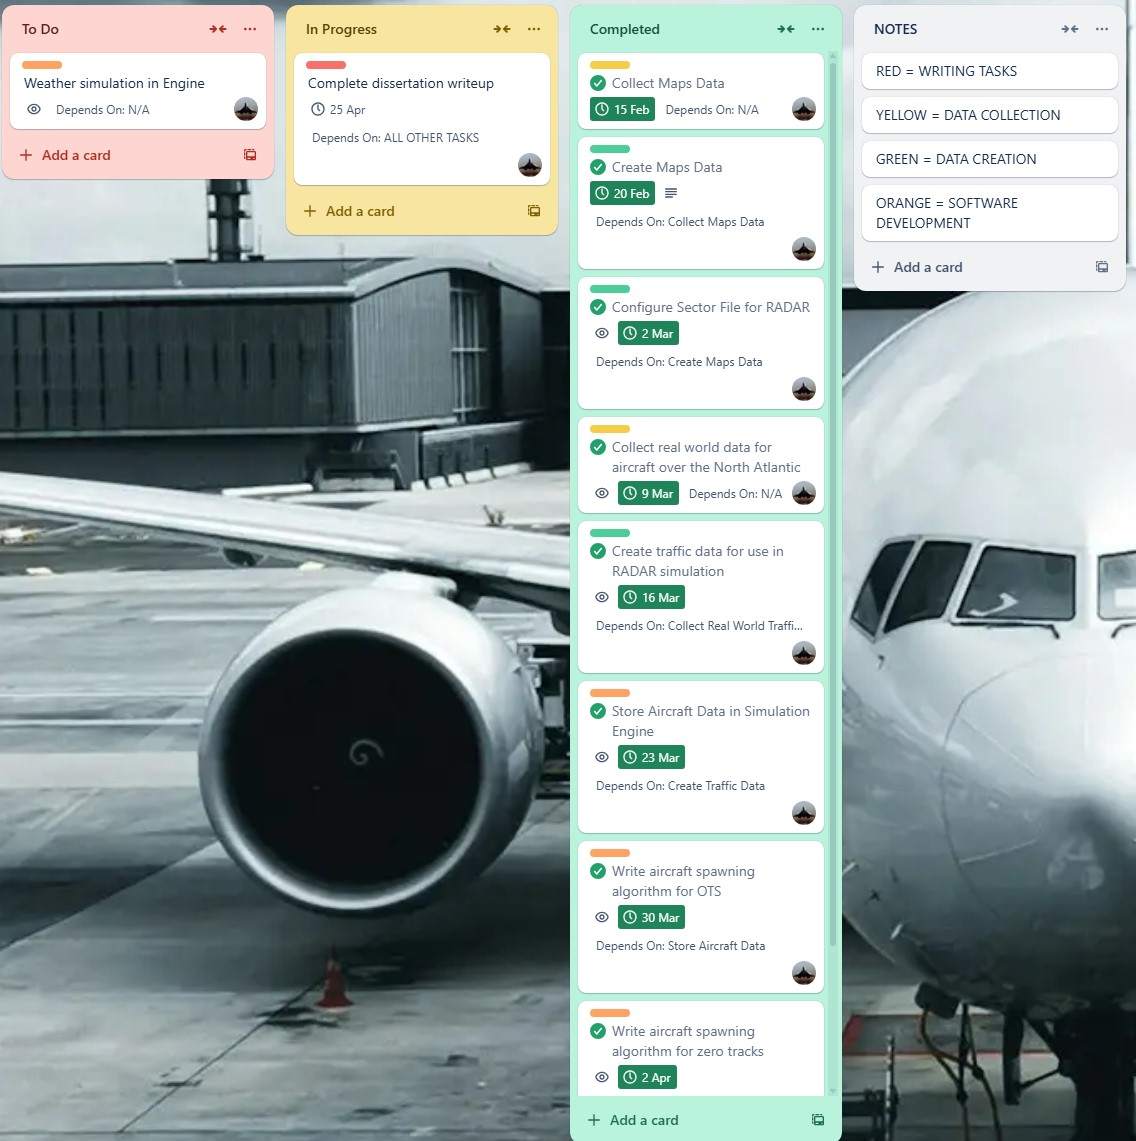
\includegraphics[width=1.1\textwidth]{pictures/Figure 1.2.jpg}    
\end{figure}

As seen in the above figure, each of the main phases of the project has a card, which can be passed between three different phases: To Do, In Progress and Completed. As well as this, each card displays the task’s due date and all other tasks that depend upon it. This tool was incredibly useful in conducting the project and ultimately ensured that it was completed on time.

When setting task due dates, the intention was to provide more time than was reasonably needed for each task. Primarily, this was done to combat delays pre-emptively while creating a stress-free environment to work in. Ultimately, this approach was very successful and kept the project running on time throughout the process.
\subsection{Literature Review Summary}
As Space-based ADS-B is very modern technology, very little literature exists that is relevant to this piece of work. Similarly, since the technology is currently undergoing testing, it has not yet been certified for commercial use, and therefore, technical information about Aireon’s satellites is limited. Therefore, the literature reviewed for this project focused on the theoretical foundations of Space-Based ADS-B, how ADS-B works and methods of air traffic management over the North Atlantic Ocean. A thematic literature review was conducted, with the goal of spotting key trends and potential gaps in the current literature.
\subsubsection{North Atlantic Tracks and OTS System}
In \textit{North Atlantic Aircraft Trajectory Optimisation}, Rodionova (and others) discuss how the OTS manages trans-atlantic flights by assigning structured routes that are east-bound in the evening (GMT) and west-bound in the morning (GMT) (\cite{OTS}). This leads to suboptimal routing for many aircraft and therefore increased flight times and higher fuel burn, which ultimately leads to higher ticket prices and greater environmental impact. This system is used because there is a lack of surveillance equipment over the ocean and so aircraft have large spacing requirements (60 NM horizontally and 1000ft vertically), while also making a position report every 15 minutes (\cite{OTS}).
\subsubsection{Technological Foundations of Space-Based ADS-B}
In \textit{Aireon Space Based ADS-B Performance Model} Garcia (and others) discuss how ADS-B evolved from World War 2 Identification Friend-Or-Foe systems (IFF) (\cite{AireonSpaceBasedADSBPerformanceModel}). Initial systems like Mode S used interrogation and reply mechanics, which were then upgraded in the 1990s to 1090ES ADS-B. This new standard of ADS-B technology allowed aircraft to automatically broadcast their GPS position, without being first interrogated; as they would have been if Mode S was being used. 

However, conventional ADS-B has two major limitations: 
\begin{enumerate}
    \item Line of sight is required,
    \item Signal range is limited to about 450 km(\cite{flightRadar}).
\end{enumerate}

In \textit{Space-Based ADS-B: Performance, Architecture and Market} Baker suggests that Space-Based ADS-B is the solution to these limitations as with a sufficient satellite constellation (in this case Aireon has 66 satellites), global coverage can be achieved, including oceanic and remote regions \cite{SpaceBasedADSBPerformanceArchitectureAndMarket}. In \textit{Aircraft Surveillance from Space: The Future of Air Traffic Control} Budroweit (and others) make a similar observation \cite{AircraftSurveillanceFromSpace}. 

Furthermore, Baker distinguishes between ADS-B and ADS-C, the later being a satellite communication based tracking tool, used for non-surveillance purposes. This is because ADS-C is limited by update intervals, making it unsuitable for real-time ATC surveillance (\cite{SpaceBasedADSBPerformanceArchitectureAndMarket}). 

\subsubsection{System Performance and Metrics}
In their respective publications, Garcia and Baker discuss that to be ICAO compliant, any ATC surveillance system must meet the following criteria (\cite{ICAO2007}):
\begin{itemize}
    \item An up-time of 99.9\% or greater per year,
    \item Less than 2 seconds of latency,
    \item Update intervals at intervals of no more than 8 seconds, at a 95-96\% confidence level.
\end{itemize}
Aireon’s system is currently the only Space-Based ADS-B provider that meets these ICAO standards; other providers currently on the market, such as Globalstar and Spire, can only meet tracking standards, and some do not offer global coverage. Aireon is able to meet these strict requirements due to its use of the Iridium-NEXT satellites, which are Low Earth Orbit (LEO) systems; their proximity to Earth reduces signal propagation times. 
\subsubsection{Implementation Challenges and Solutions}
Garcia suggests that there are two major challenges when implementing Space-Based ADS-B systems. 

First of all, signal interference from older systems, like Mode S and IFF, which cause False Replies Uncorrelated In Time, or FRUIT, errors (\cite{AireonSpaceBasedADSBPerformanceModel}). These errors mean that the newer system, in this case Aireon’s Space-Based ADS-B system, spends time processing old, useless data, and therefore ignores real signals that are important. 

Secondly, overlapping satellite coverage can lead to signal garbling in areas of high traffic density (\cite{AireonSpaceBasedADSBPerformanceModel}). This means that signals may never reach a satellite, or possibly arrive in an unreadable state. 

Baker says that Aireon uses probabilistic modelling to combat both of these problems. This essentially involves mathematically predicting when a message is expected to be received by a satellite and what it is expected to say (\cite{SpaceBasedADSBPerformanceArchitectureAndMarket}). This method can be used to reconstruct an unreadable signal or replace a signal that was never received. 


\subsubsection{Applications and Market Implications}
As suggested by Garcia and Baker, the primary application of Space-Based ADS-B is in air traffic surveillance, providing real-time position data for collision prevention and traffic management (\cite{SpaceBasedADSBPerformanceArchitectureAndMarket} and \cite{AireonSpaceBasedADSBPerformanceModel}). This differs from solutions currently available on the market as Space-Based ADS-B can monitor aircraft in areas of the planet not currently accessible to Air Traffic Controllers, such as Oceanic regions and remote areas. An article published by Pyramid Media Group Inc. reinforces this idea and that the implementation of Space-Based ADS-B will eventually lead to improved efficiency and capacity over the North Atlantic Ocean (once it replaces the OTS) \cite{SpaceBasedADSBChangesFlying}. 

This, however, is not the only use-case for Space-Based ADS-B. The technology can also be used to aid in aircraft incident investigations, especially those that occur in remote areas. Additionally, airlines can use the technology to track their fleet of aircraft for operational planning and information. Both of these use cases do not require the level of fidelity that aircraft surveillance systems must meet. Instead, they can comply with Aircraft Tracking solutions, such as those provided by Globalstar and Spire.  

\subsubsection{Gaps in the Literature}
While conducting the literature review, it became clear that no publication attempted to discuss Space-Based ADS-B’s impact on Air Traffic Management over the North Atlantic ocean using numerical and factual data. The article published by Pyramid Media Group Inc. quoted a NATS air traffic controller as saying the testing of Aireon’s system was “transformational” and resulted in aircraft saving time, money, fuel and therefore fewer emissions (\cite{SpaceBasedADSBChangesFlying}). Still, there was no attempt to quantify this claim, however logical it may seem. This gap will attempt to be filled by the research and simulations conducted in this paper. 
\subsubsection{Final Summary}
The literature review conducted finds that Space-Based ADS-B is a significant technological evolution with transformative potential, especially over remote areas. Currently, Aireon is the only provider that meets ICAO standards, and therefore, the testing of this technology is limited to just the North Atlantic region under the supervision of NATS and Nav Canada. 

The paper written by Garica (and others), \textit{Aireon Space-Based ADS-B Performance Model} was produced by a team from Aireon and therefore it is important to discuss if any bias is present. While there is a reasonable expectation for the paper to have some bias, overall it makes claims very similar to the other pieces of work that have previously been discussed and therefore it is a useful body of work to consider for this project. 

Based on this literature review, the research outcome for this project was decided to investigate, by quantifying, the actual usefulness of Aireon’s Space-Based ADS-B system, in terms of creating more efficient air traffic and airspace management over the North Atlantic Ocean. 

\newpage
\section{Methodology}
The goal of this research project is to compare two different methods of air traffic management, in particular over the North Atlantic Ocean. Since NATS and Nav Canada do not publish data on when they operate “zero tracks”, real-world data cannot be directly used to make this comparison. Therefore, it was decided that the best approach would be to create a simulation engine, which could be used to make a comparison. For the simulation engine to be a useful method of comparison, it is important to build it using real-world data and statistics.

With this in mind, much of the methodology will explore how the simulation engine was built and then how it was calibrated to match how aircraft behave over the North Atlantic Ocean in reality. The engine was not created entirely from scratch for the project; rather, an existing, in-development RADAR application created by Terminal2Solutions (\cite{T2}) was sourced. The product produced by Terminal2Solutions provided the basic framework, which was then customised and built upon to the required specifications for this project. This application was provided voluntarily and at no expense to the researcher. The following subchapters will explore how this application was modified and expanded for the purposes of this project.   
\subsection{Simulation Engine Data Creation and Collection}
In order for the application display to be useful and readable, especially to a person unfamiliar with the geography of navigation aids on either side of the Atlantic ocean, it was decided to import geographical map data into the software. The following subchapter will explore how that was accomplished.
\subsubsection{Collection and Formatting Maps Data}
A charitable organisation called Natural Earth (\cite{NaturalEarth}) provides open-source geographical data for the entire world, which includes everything from maps of roads and cities, to basic coastline data. For the purposes of this project, a map only needs to display the coastline of counties, specifically,
\begin{enumerate}
    \item The United Kingdom,
    \item The Republic of Ireland,
    \item Iceland,
    \item The entirety of western Europe, including Scandinavia and Greenland,
    \item The eastern seaboard of the United States of America and Canada. 
\end{enumerate}
However, Natural Earth provides this data for the whole globe, not specific countries. Therefore, a resolution of 1:50m was selected and then information was extracted from the map of the world using a piece of open-source software called QGis (\cite{QGIS}). Figure 2.1 shows the coastline data for the entire world, from Natural Earth, imported inside of QGis. 

\begin{figure}[H]
    \caption{Coastline data for the entire Earth, imported inside of QGis.}
    \label{fig:2.1}
    \centering
    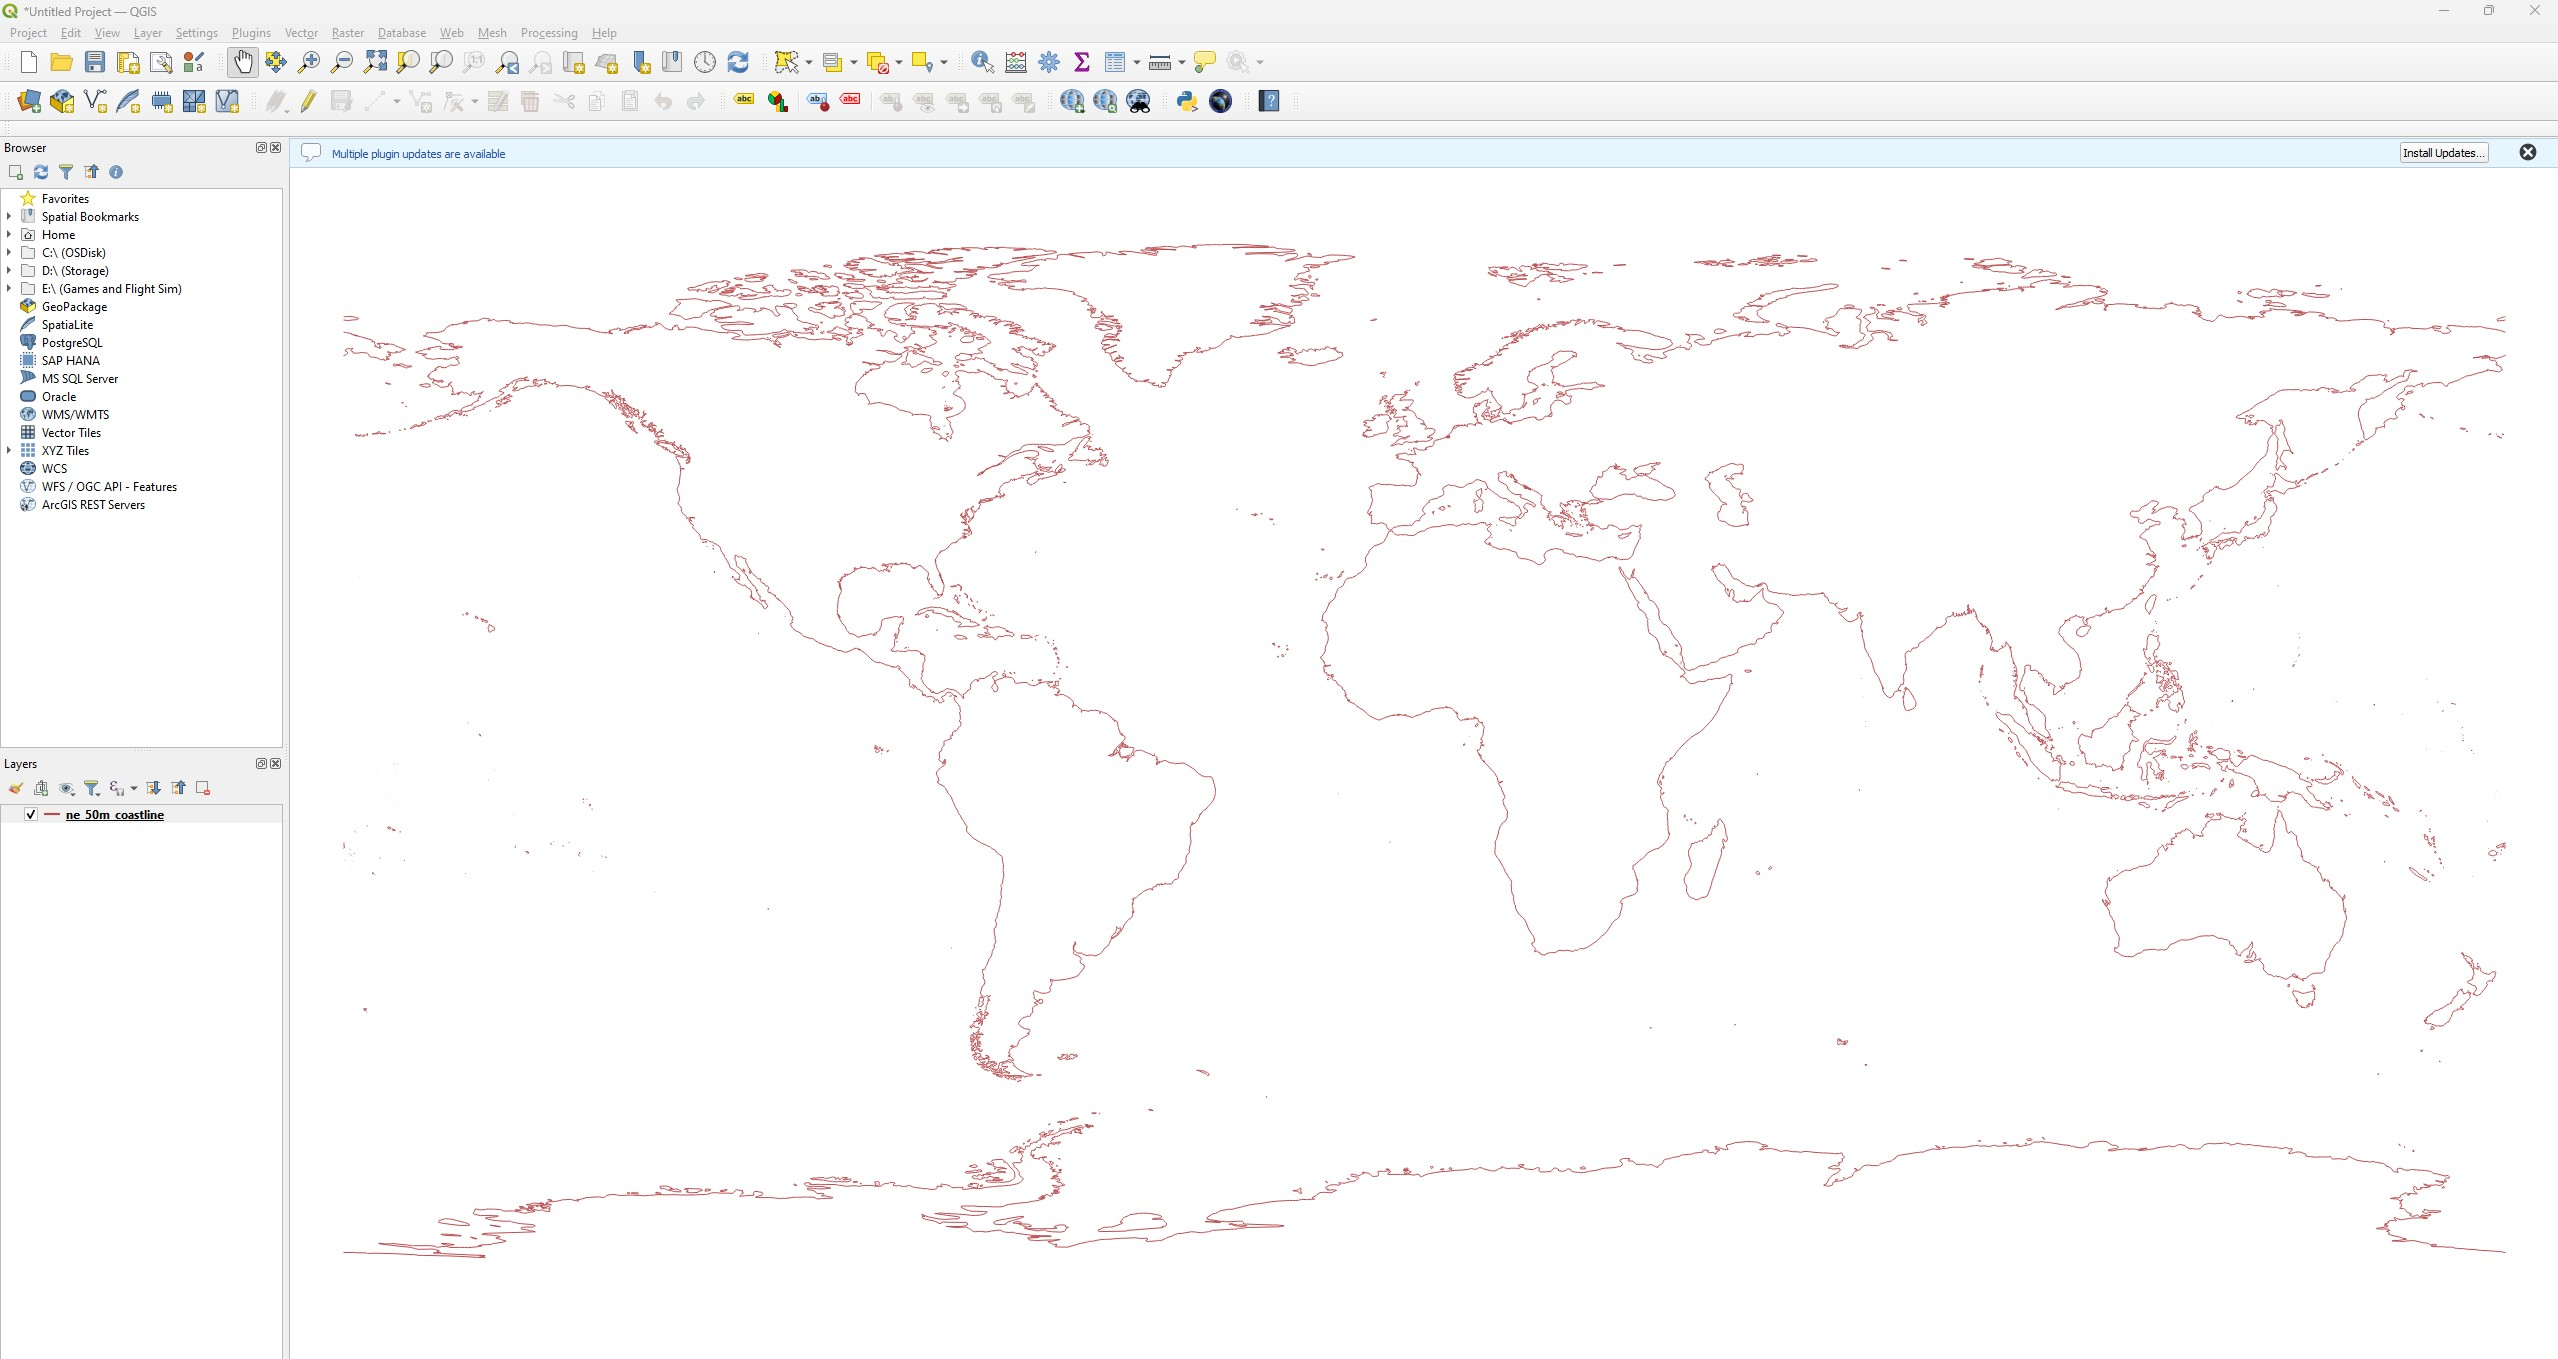
\includegraphics[width=1.1\textwidth]{pictures/Figure 2.1 FYP.jpg}    
\end{figure}

QGis is a useful tool as it allows specific regions, and the data belonging to that region to be extracted. At this point, it is important to understand the details behind the coastline data. Simply put, the image seen in Figure 2.1 is created by drawing a straight line between two coordinates in latitude and longitude. Each individual point is spaced 50m away from the others, hence the ratio mentioned earlier. The RADAR software that is used for this project stores map data in a very similar way, so the goal of this process is to extract a list of coordinates which the software can then draw lines between to create a complex shape, in this case, the outline of a land mass. The map shown in Figure 2.1 contains hundreds of thousands of these coordinate pairs, which is why QGis is used to isolate just the regions of interest - it is simply not practical to complete this step by hand. For example, Figure 2.2 shows the isolated map data for the United Kingdom, the Republic of Ireland and the smaller Islands that comprise the British Isles. 

\begin{figure}[H]
    \caption{Coastline data for the British Isles, imported inside of QGis.}
    \label{fig:2.2}
    \centering
    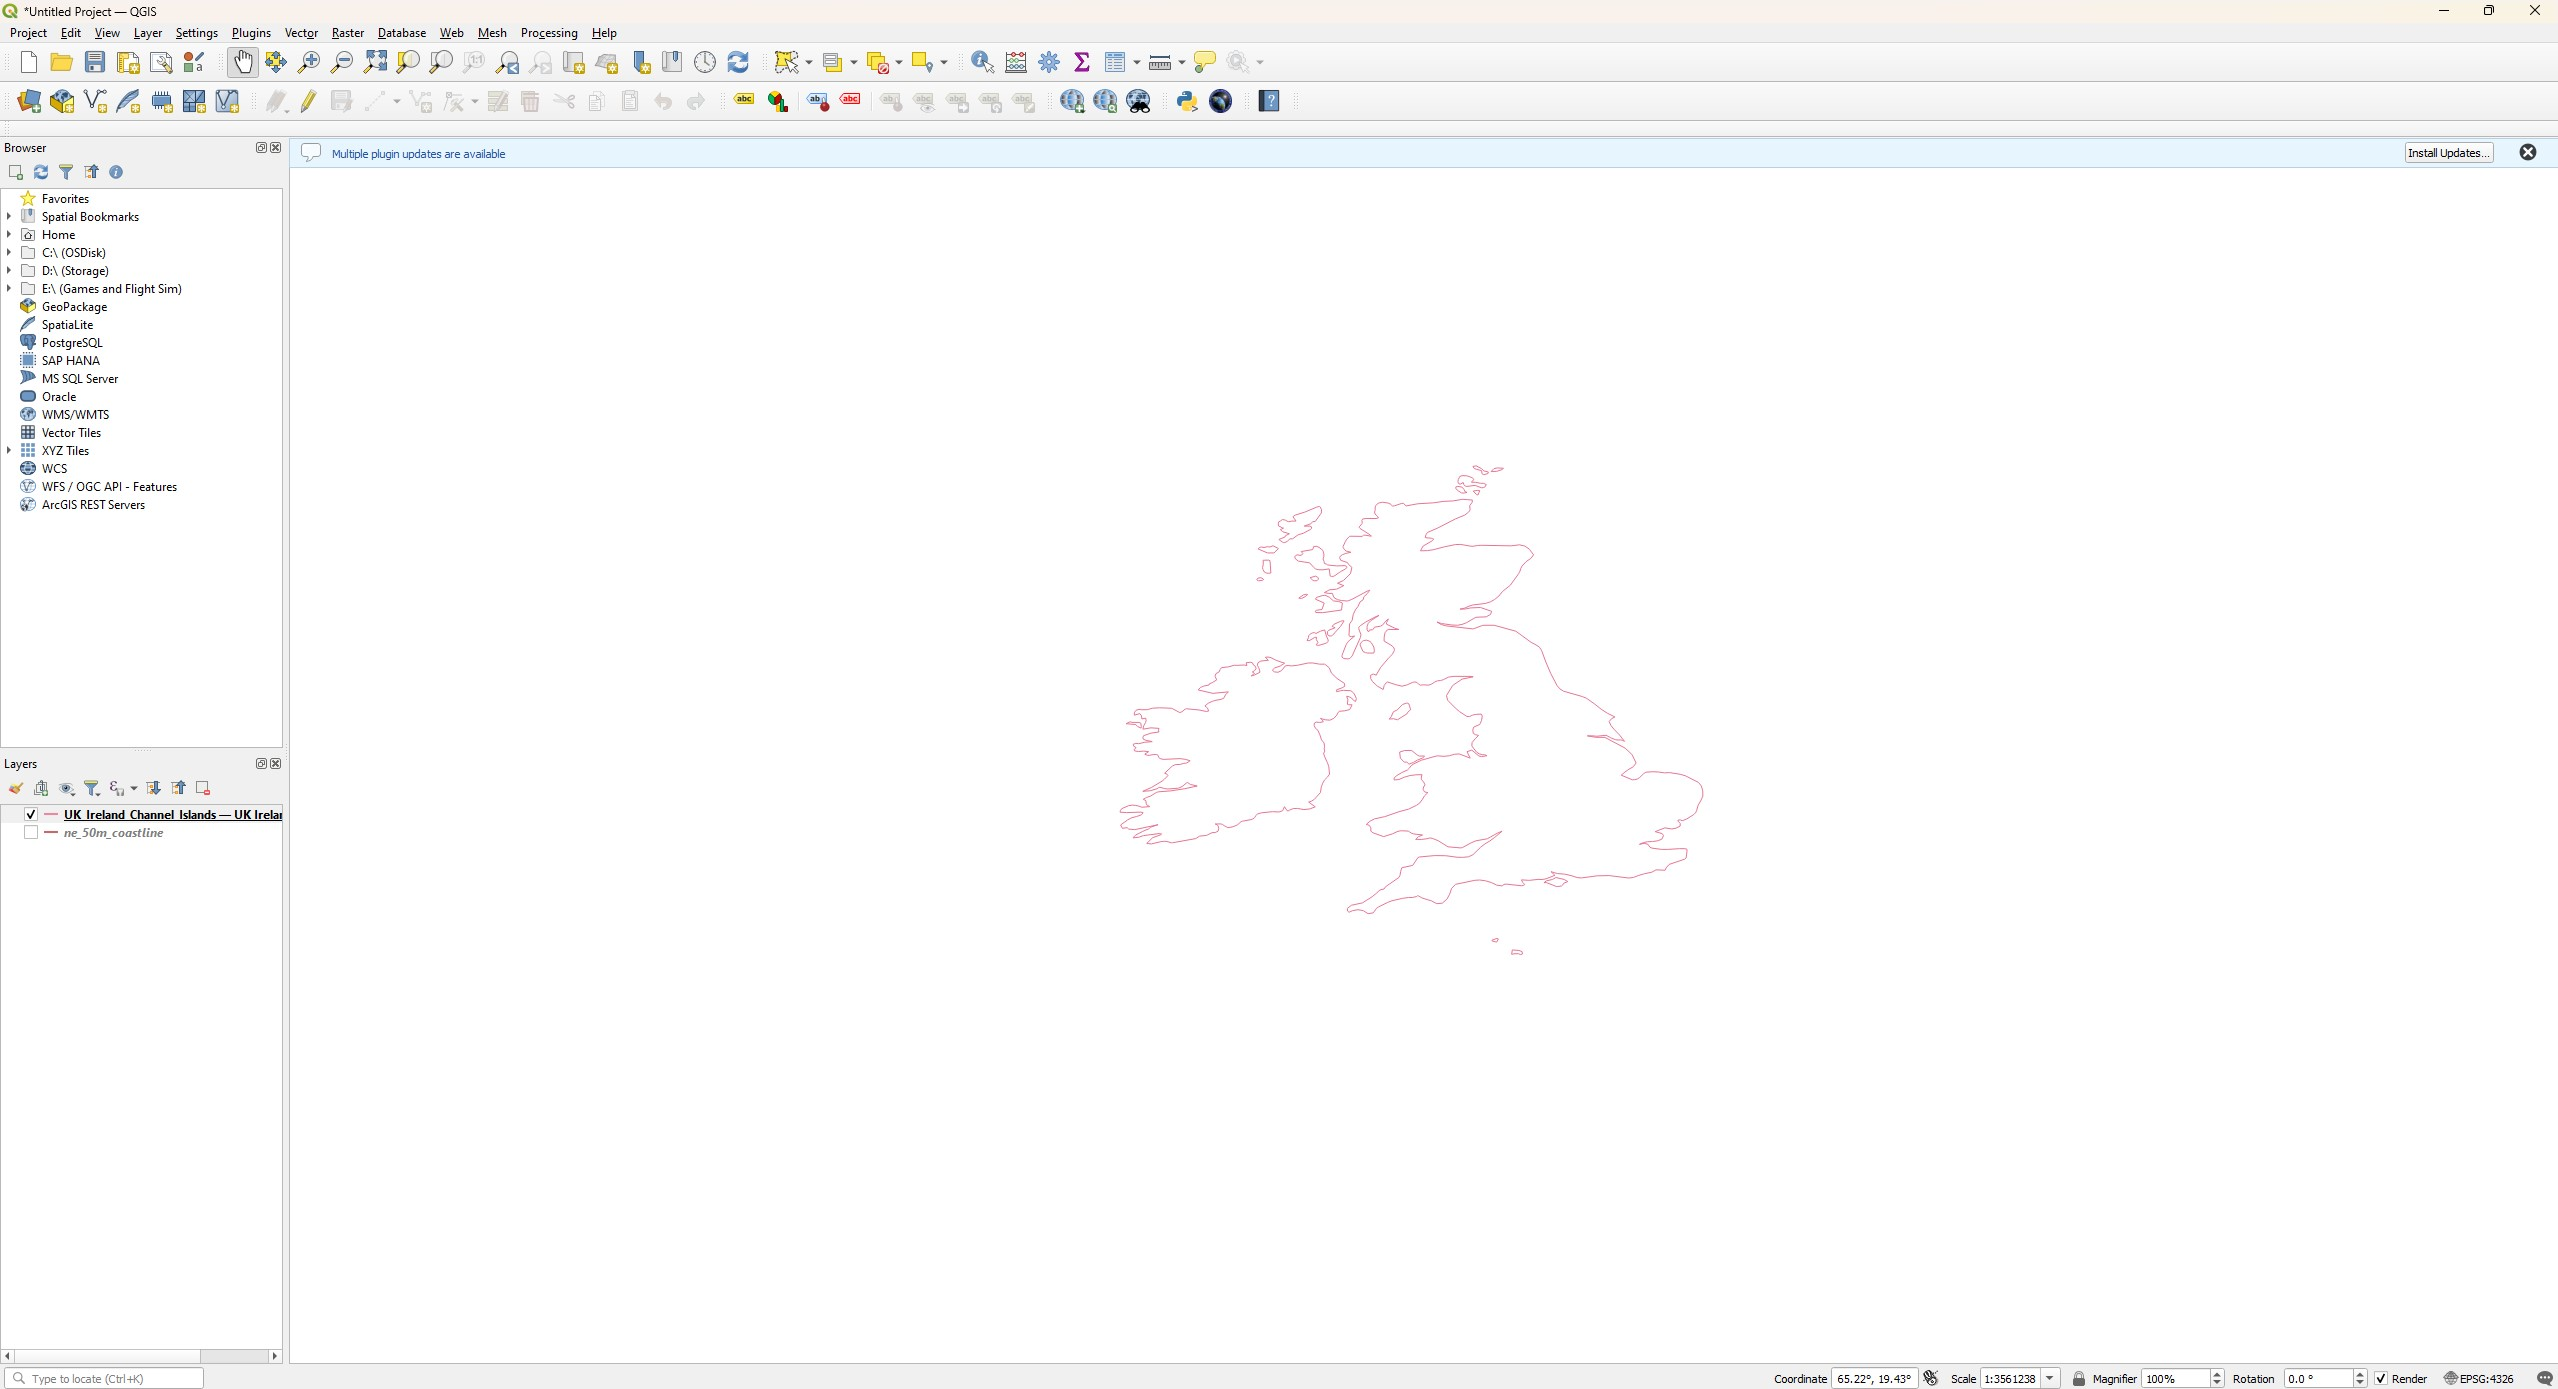
\includegraphics[width=1.1\textwidth]{pictures/Figure 2.2 FYP.jpg}    
\end{figure}

For the purposes of this subchapter, the entire process will be shown to import the British Isles into the RADAR software, all other landmasses were produced in an identical manner. 

Once the data, as seen in Figure 2.2, has been isolated, it needs to be imported into the RADAR software. Unfortunately, this is not a straightforward process due to the different ways data is stored between QGis and the RADAR. QGis outputs the data in a .geojson file type, a subsection of this data can be seen in Figure 2.3. 

\begin{figure}[H]
    \caption{A subsection of GEOJSON data for the British Isles. The contents of this data is not important, the aim is to show the vast nature of the data.}
    \label{fig:2.3}
    \centering
    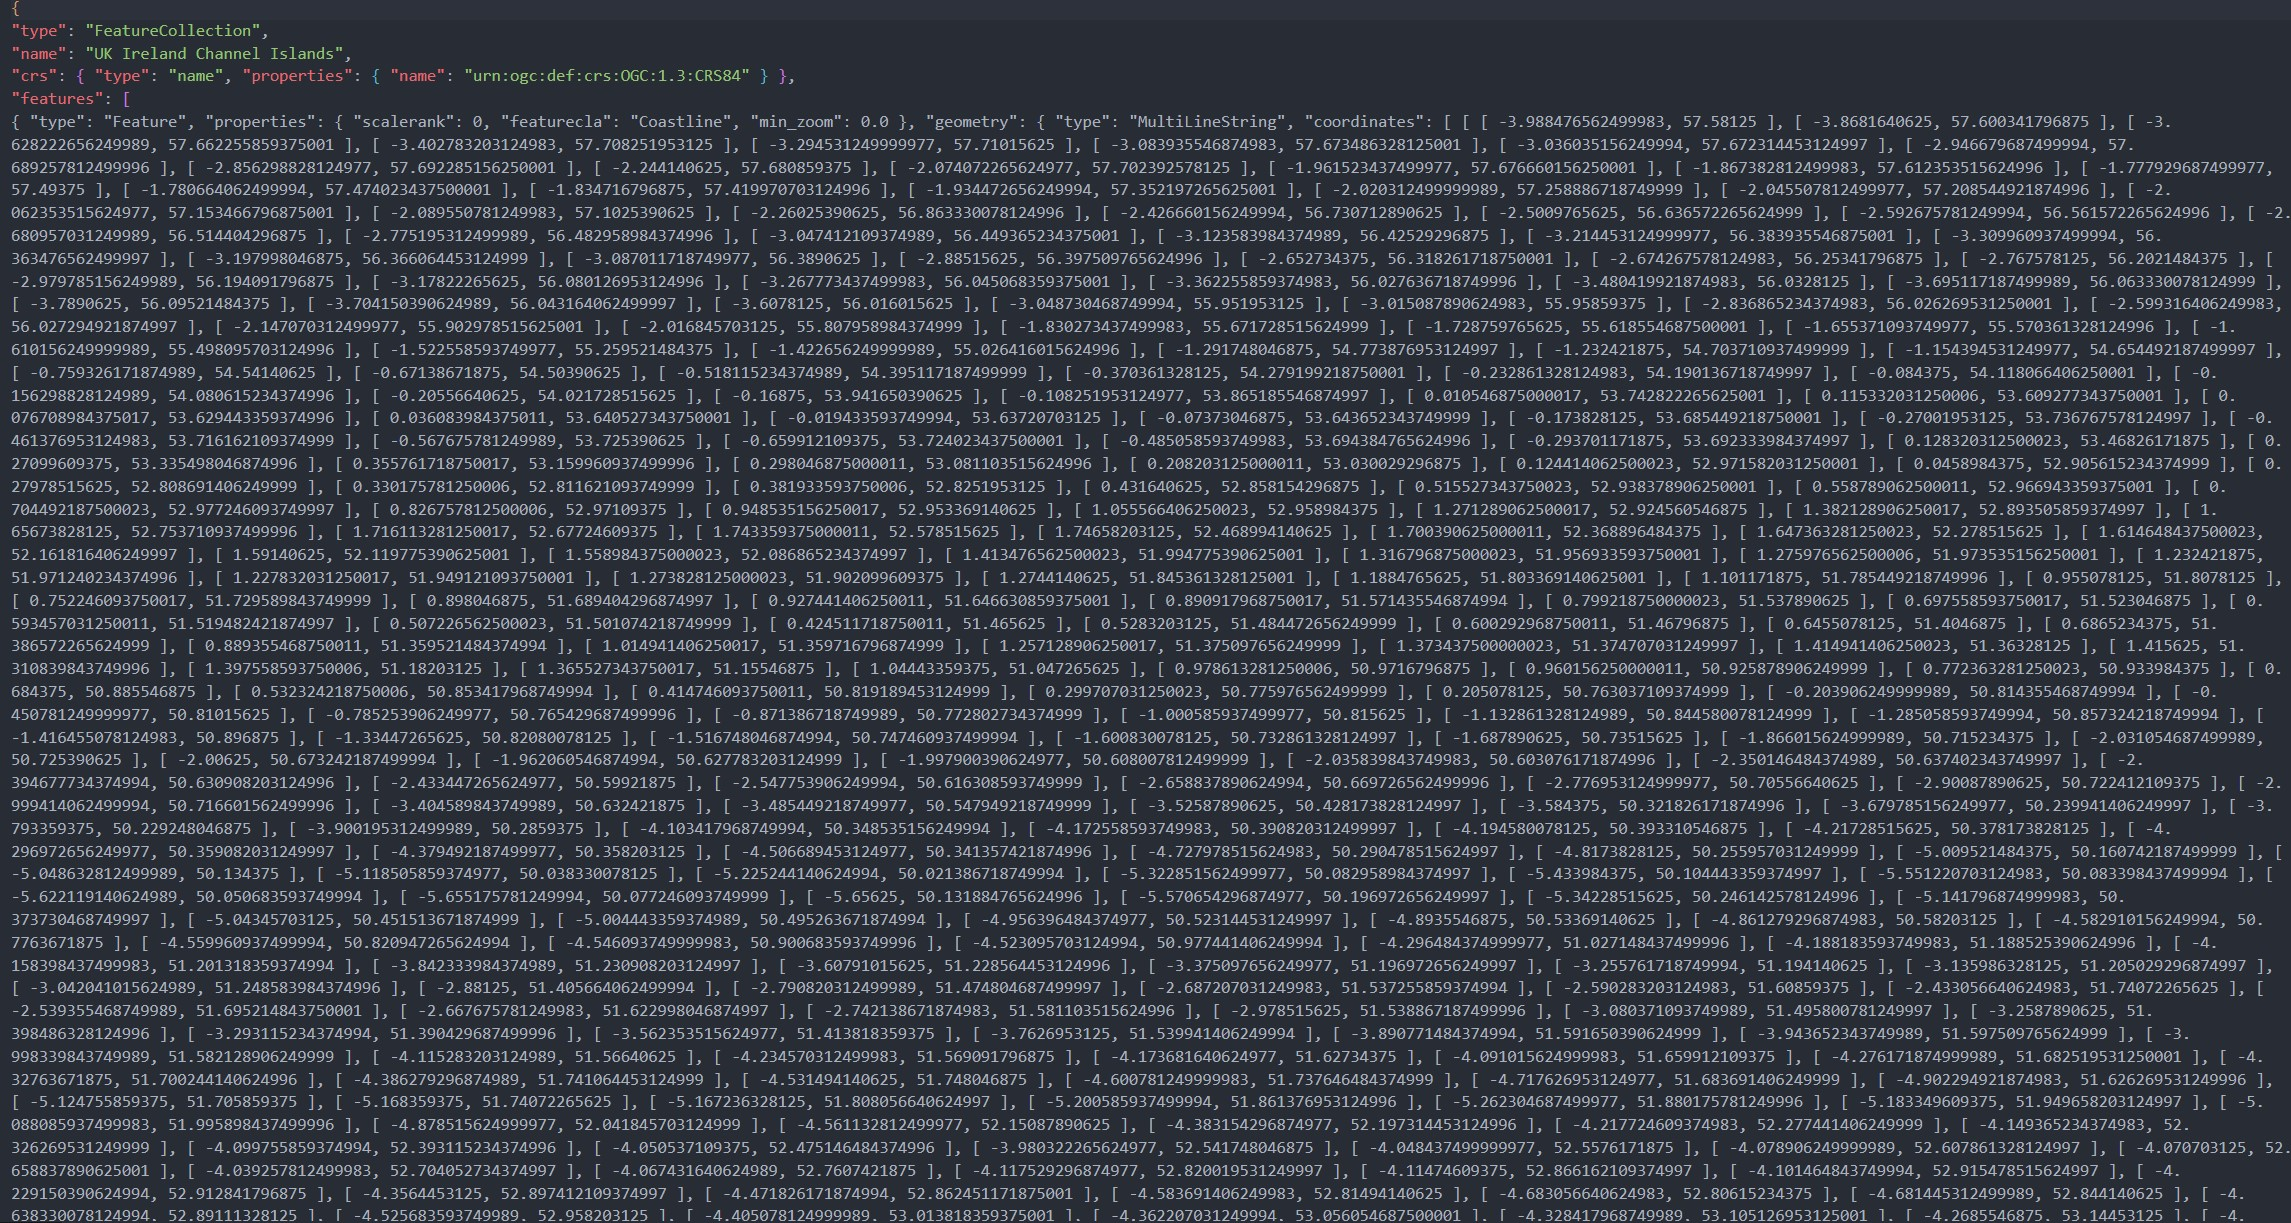
\includegraphics[width=1.1\textwidth]{pictures/Figure 2.3 FYP.jpg}    
\end{figure}

The first problem is that RADAR expects to receive coordinates of latitude and longitude in the format DDDMMSS, not in decimal format as shown here. Additionally, the format of the data needs to change from a .geojson file to an .xml file. The researcher did not make these decisions; it is simply a requirement of the RADAR software, which must be conformed to. In particular, the RADAR software expects to receive map data in the format shown in Figure 2.4.

\begin{figure}[H]
    \caption{Expected format of Coastline data for the RADAR software; its quite different from the format provided in the GEOJSON file.}
    \label{fig:2.4}
    \centering
    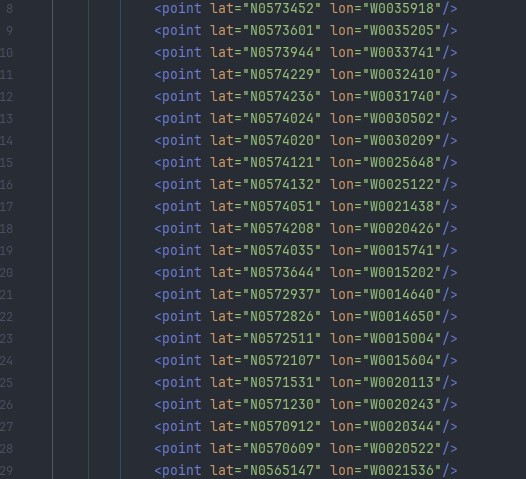
\includegraphics[width=1.1\textwidth]{pictures/Figure 2.4 FYP.jpg}    
\end{figure}

Due to the vast amount of data that had to be handled for this phase of the project, it was decided to write two simple scripts in Python3. The first script took the output from QGis shown in Figure 2.3 and converted all the coordinates from radians to DDDMMSS as well as eliminating the unnecessary data from the original .geojson file. This produces an output, a subsection of which can be seen in Figure 2.5.

\begin{figure}[H]
    \caption{A subsection of the GEOJSON data trimmed down by the first Python3 script.}
    \label{fig:2.5}
    \centering
    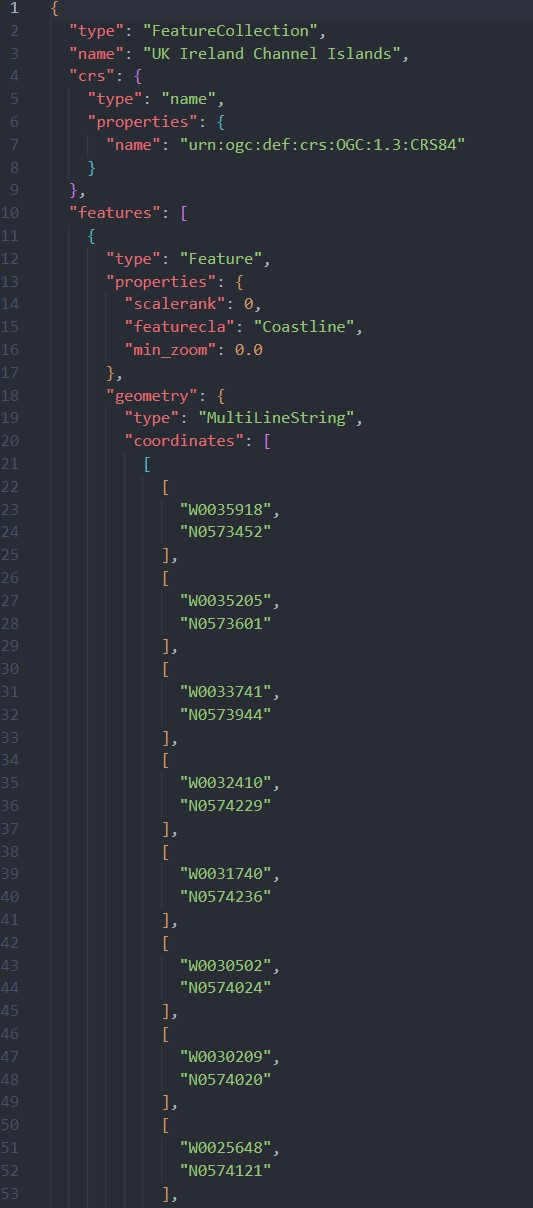
\includegraphics[width=1.1\textwidth]{pictures/Figure 2.5 FYP.jpg}    
\end{figure}

At this stage, very obvious coordinates start to appear in the file; these now need to be manipulated to be put in the format shown in Figure 2.4. This was the purpose of the second Python3 script. This puts the data into the correct format, which can then be injected into the RADAR software, giving an outcome as seen in Figure 2.6. 

\begin{figure}[H]
    \caption{Finalised coastline data inside of the RADAR software.}
    \label{fig:2.6}
    \centering
    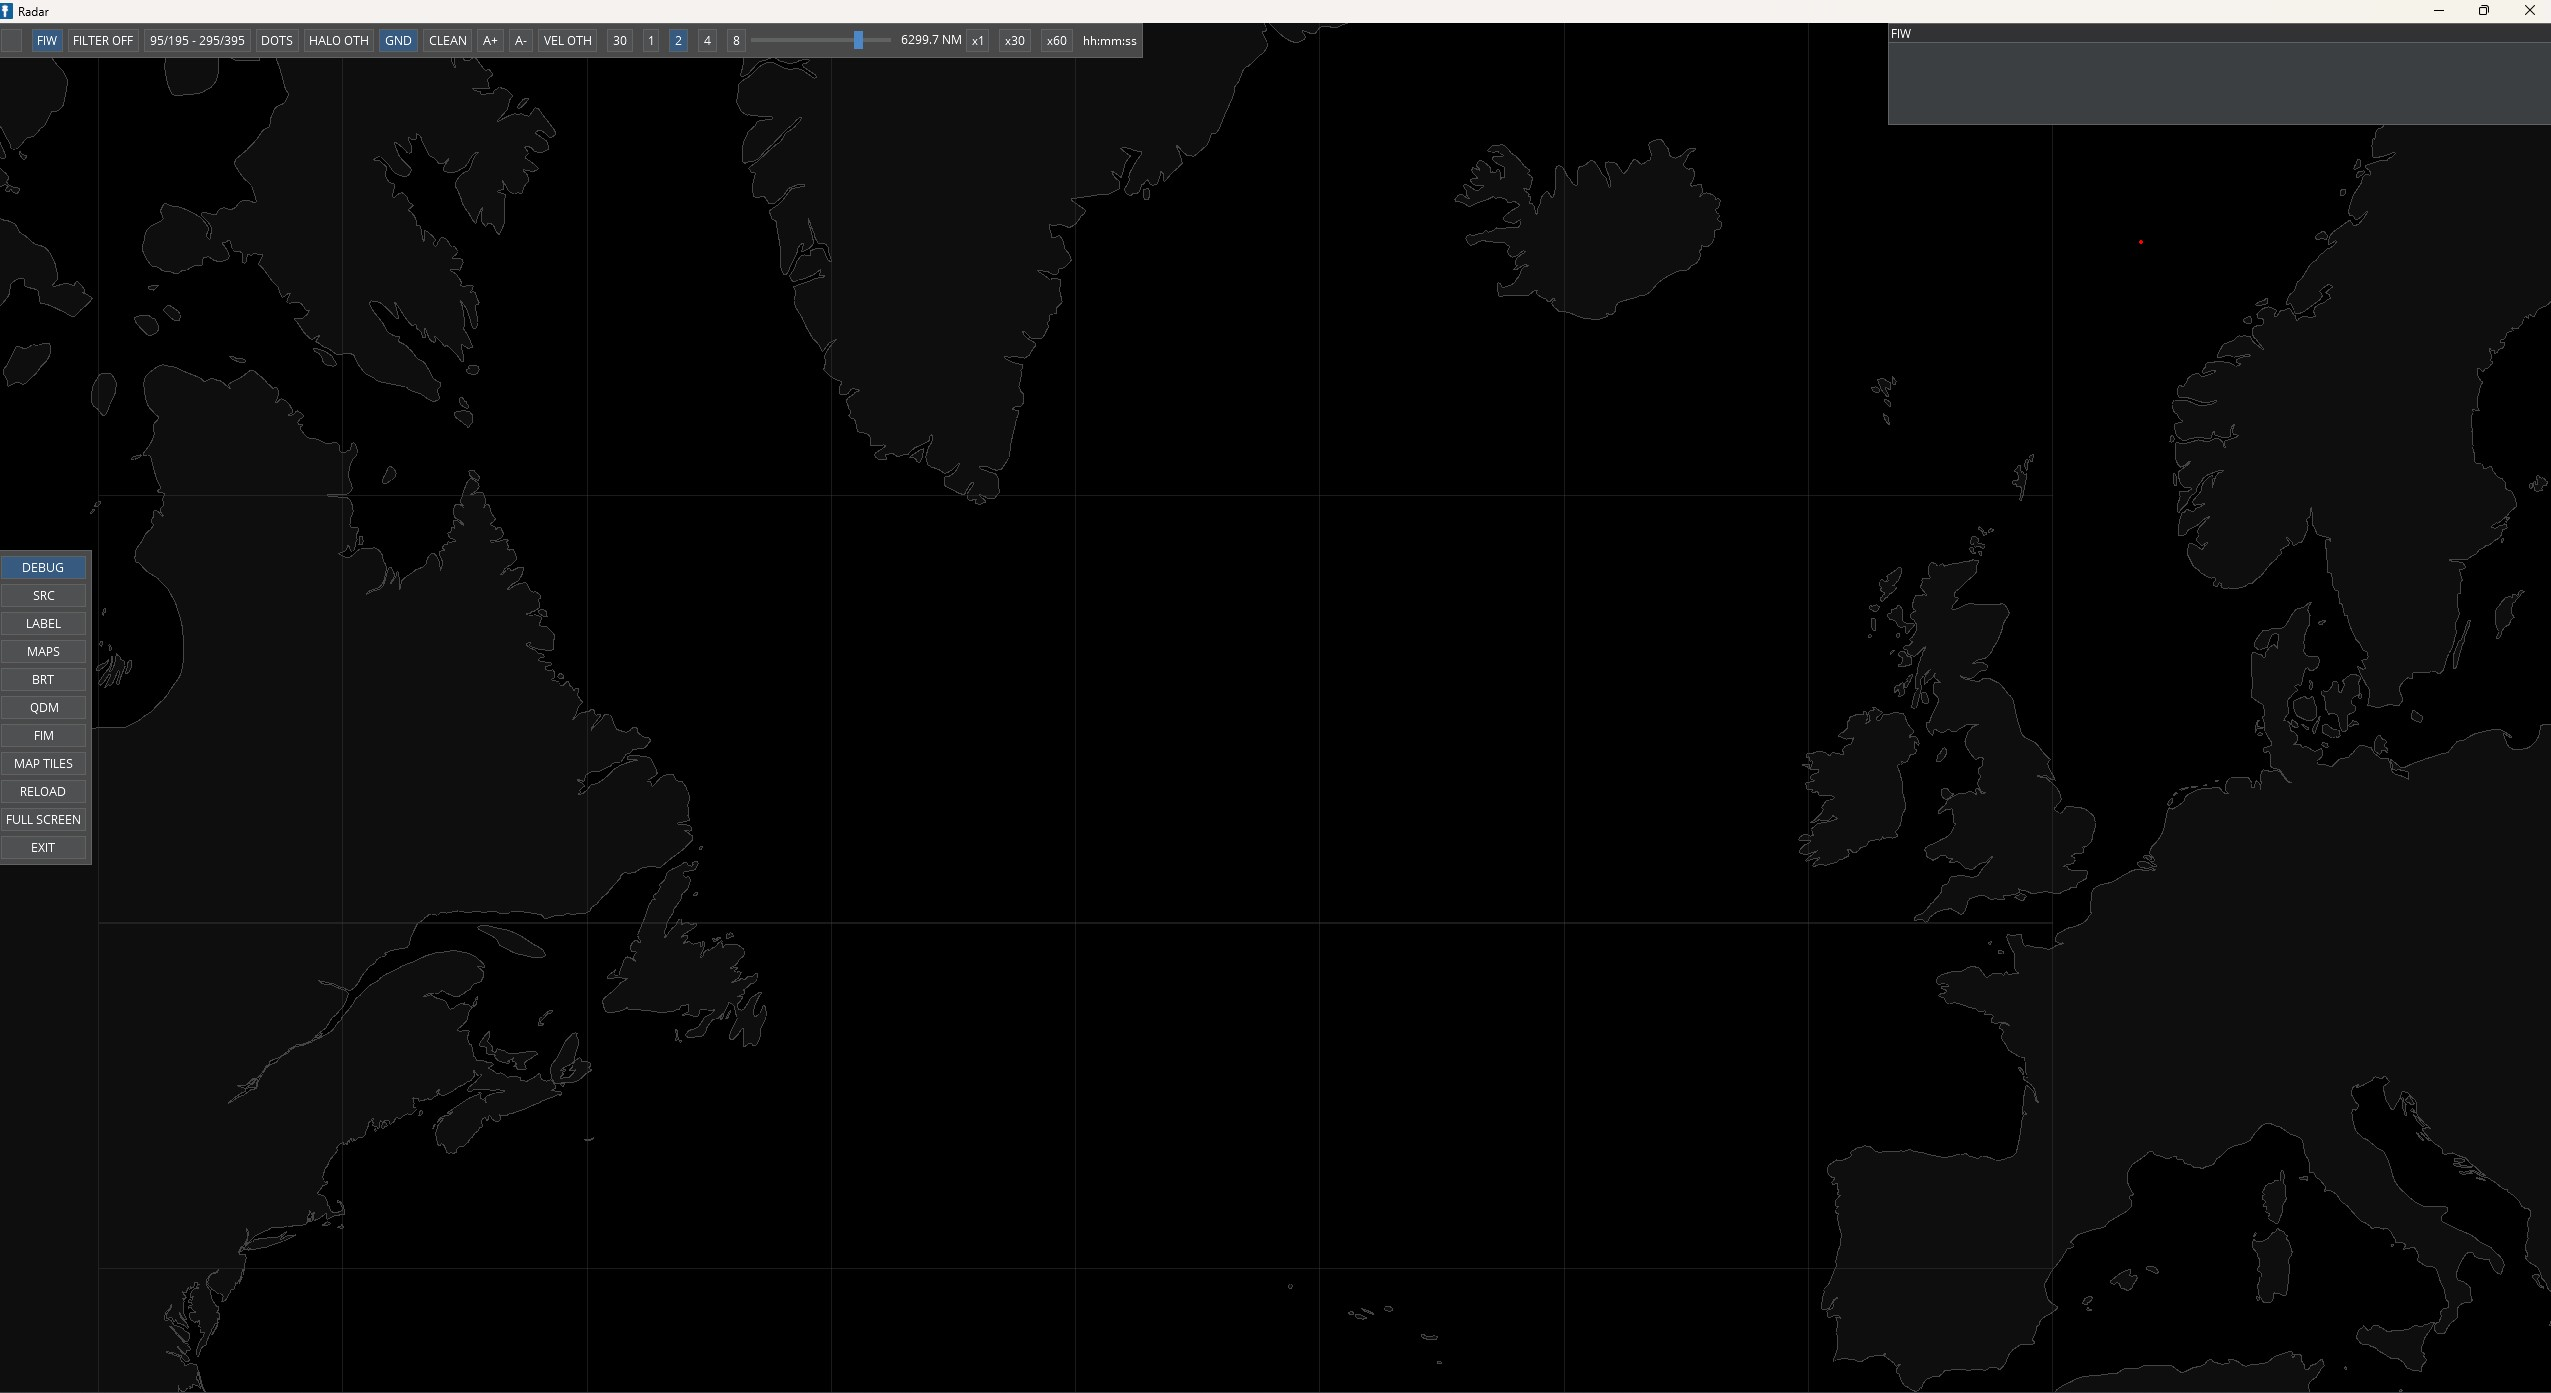
\includegraphics[width=1.1\textwidth]{pictures/Figure 2.6 FYP.jpg}    
\end{figure}

To create this image, 16912 lines of .xml map data were created, using the two Python3 scripts previously mentioned. Both of these scripts, in their entirety, can be found in Appendix A. While this data is not strictly necessary for the project to be completed successfully (aircraft can be simulated on a blank RADAR), it adds much-needed context for people who are not as aware of the geography of the region, or the position of Nav-adis either side of the Atlantic, making this body of work easier to understand. 

\subsubsection{Sector File Creation}
In the context of the RADAR software, a Sector file displays all the aviation information and data on top of geographical maps. This data was created by hand, from sources published by various international and national organisations responsible for maintaining air traffic services. This data is vitally important as the “AI” aircraft that will eventually be simulated uses this data to navigate across the airspace. Figure 2.7 shows the RADAR screen depicted in Figure 2.6, but with the sector file information also displayed. 

\begin{figure}[H]
    \caption{Finalised sector file displayed in the RADAR software. This image shows all relevant Nav-aids and oceanic tracks overlayed on the coastline data.}
    \label{fig:2.7}
    \centering
    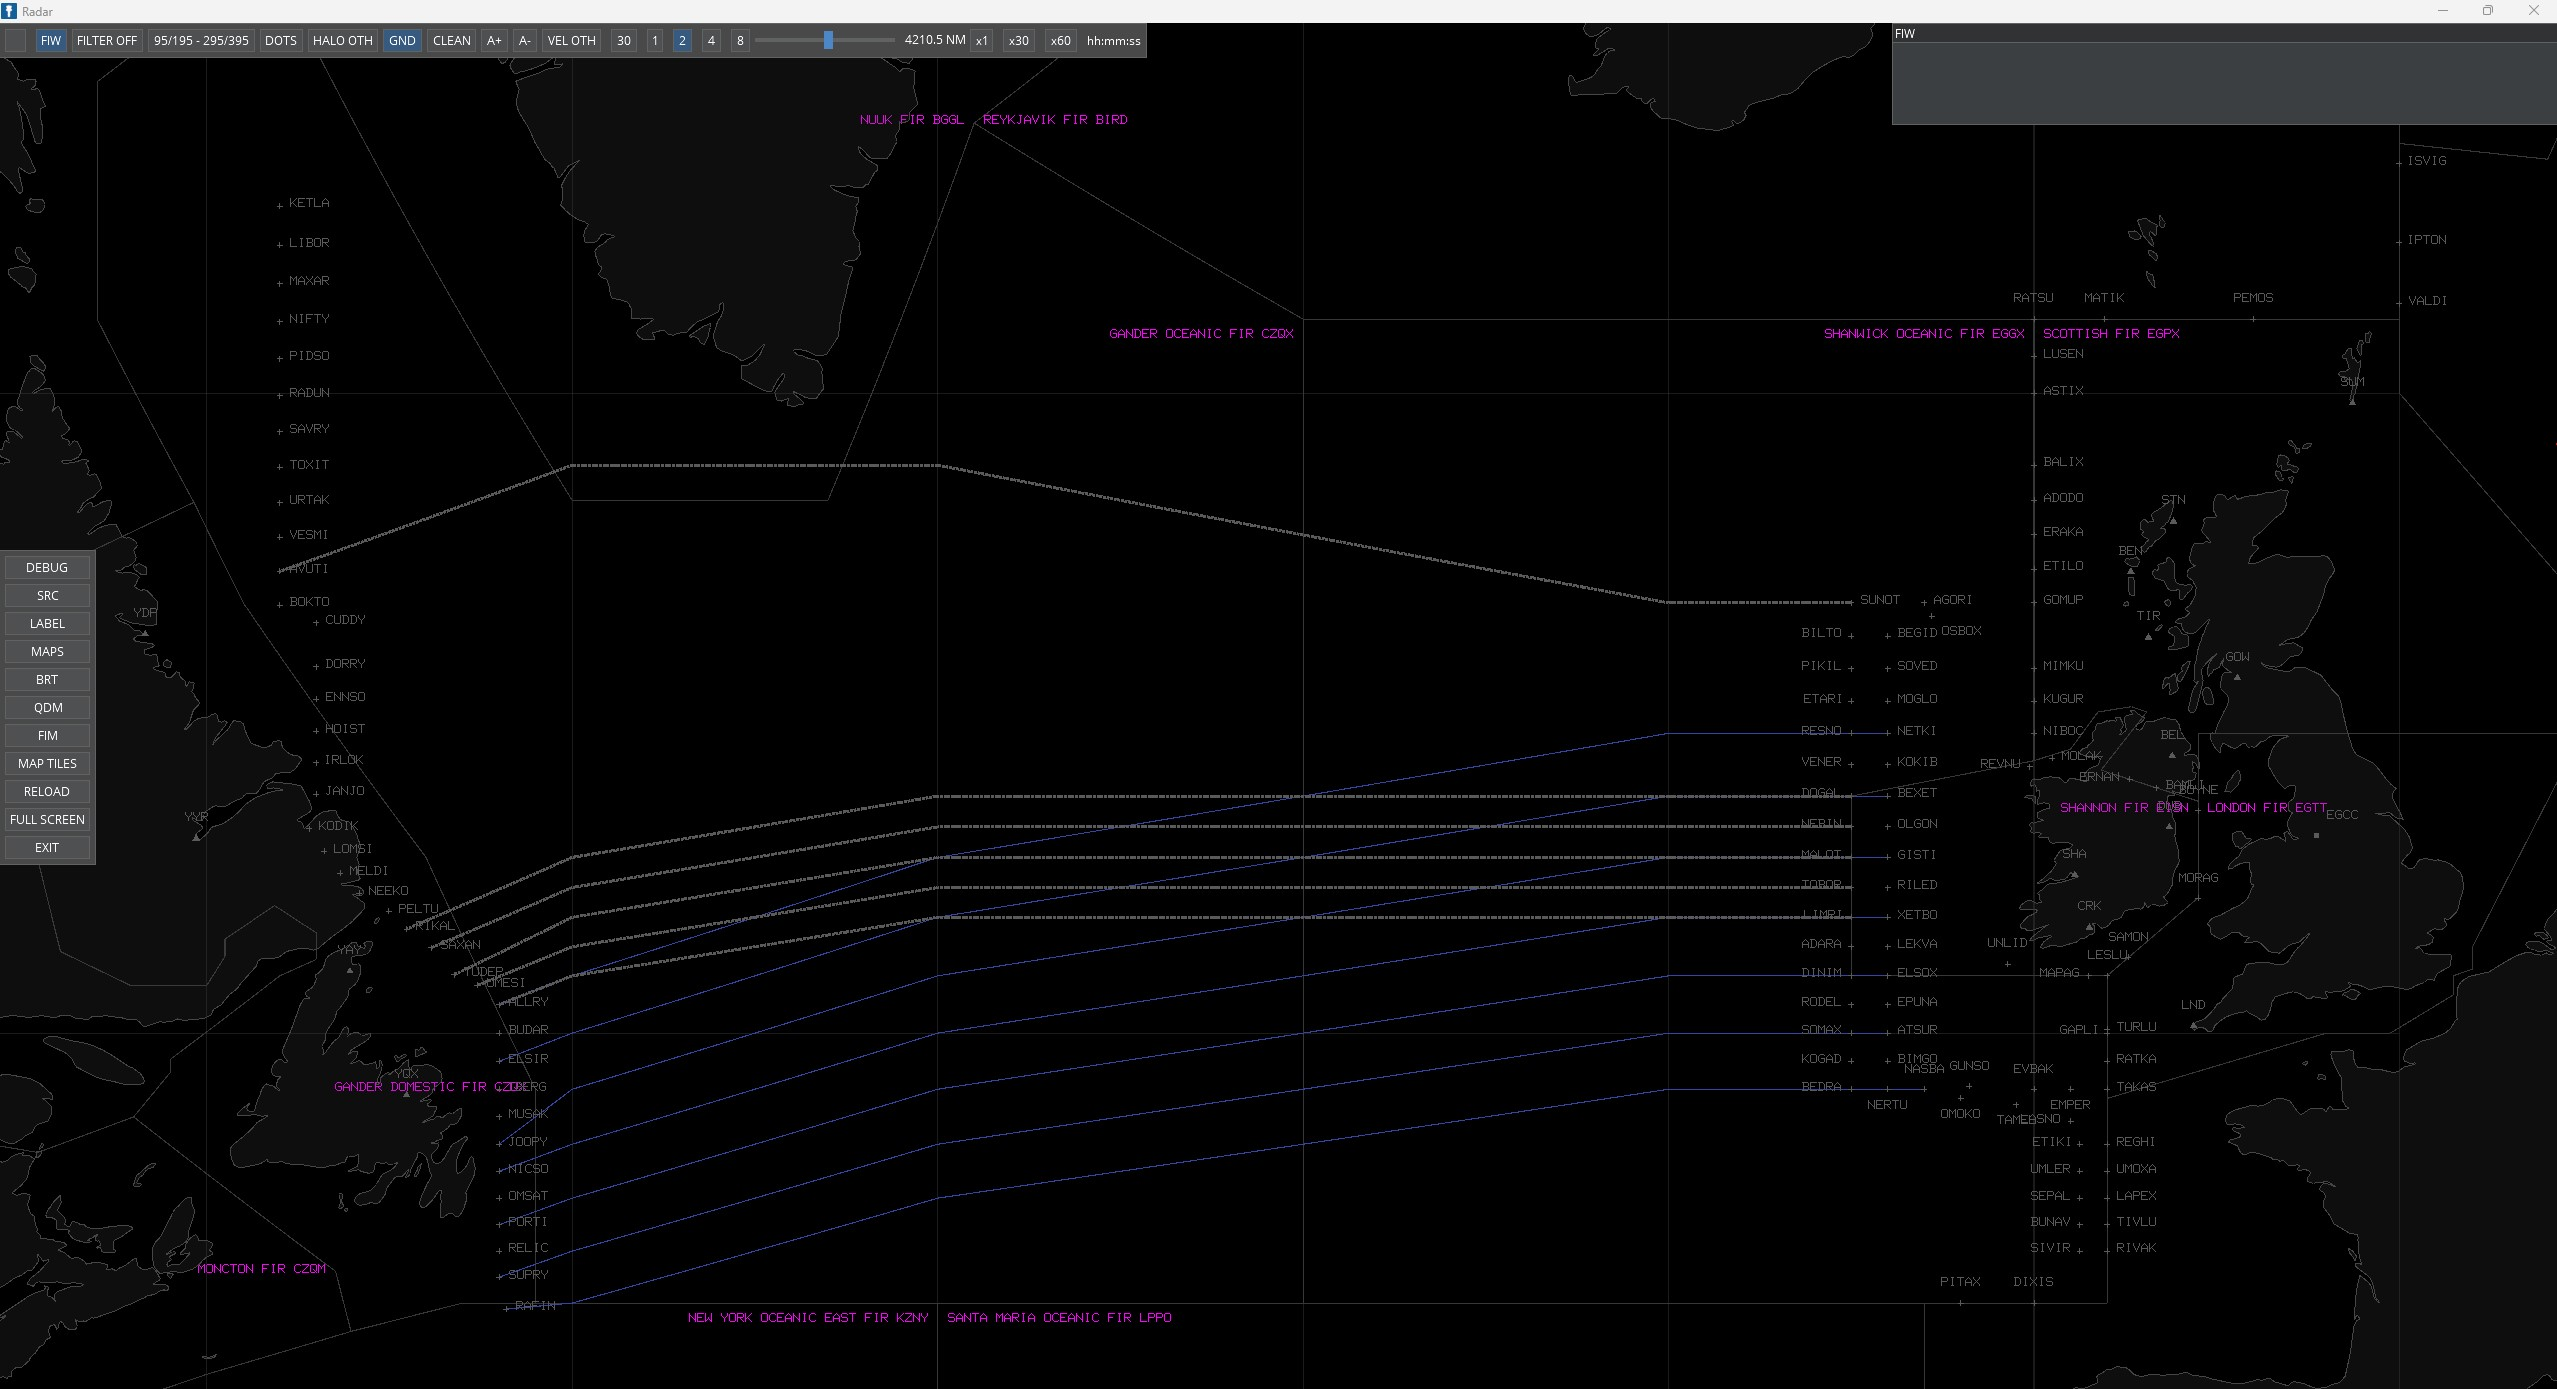
\includegraphics[width=1.1\textwidth]{pictures/Figure 2.7 FYP.jpg}    
\end{figure}

Information shown in this image includes:
\begin{itemize}
    \item Flight Information Region (FIR) boundaries, 
    \item Oceanic Entry/Exit Points (displayed as a cross with their respective names), 
    \item A small selection of VORs (displayed as triangles with their 3 character ICAO definitions),
    \item The North Atlantic Oceanic tracks in use on April 7th 2025:
    \begin{itemize}
        \item Grey tracks operate from Europe to the United States, 
        \item Blue tracks operate from the United States to Europe.
    \end{itemize}
\end{itemize}

All of the FIR region boundaries were sourced from ICAO and processed identically to the geographical coastline data as discussed in the previous subchapter (\cite{ICAO_FIR}). Whereas, all the navigation aids (entry/exit points and VORs) were obtained from the FAA’s chart of the North Atlantic Ocean from the most recent AIRAC Cycle (\cite{FAA_DEC}) and the North Atlantic Tracks were obtained from the FAA’s NAT track publisher(\cite{FAA_NAT}). 

As this data volume is much smaller than the geographical data, it was hand-formatted in .xml files in a format required by the RADAR software. 

\subsubsection{Air Traffic Data}
Now that the RADAR software has been configured, aircraft data needs to be created. So that the traffic can be made as realistic as possible, real-world air traffic over the North Atlantic Ocean was monitored over a 24-hour period. This subsection will explore how the air traffic was monitored and how it became useful for the overall simulation that was conducted.

The Flight Aware AeroAPI (\cite{FlightAwareAeroAPI}) was used to automatically monitor live air traffic over the North Atlantic Ocean. To achieve this, a third Python script was developed (you can find this in Appendix B). This script had a very basic function; every hour, it queried the AeroAPI to get a list of all aircraft over the North Atlantic Ocean at that given time. Specific data regarding each aircraft was also obtained, such as the aircraft type and the destination and arrival airports. With this information in hand, the simulation engine can be tuned to ensure that it is representative of an average day’s traffic over the North Atlantic. 

It is important to specify that since the AeroAPI depends on ADS-B signals, it is not always 100\% effective. In fact, sometimes data cannot be communicated, which may result in an unknown parameter for some tracked aircraft. 

However, in total, 1476 aircraft were captured throughout the 24-hour period. Table 2.1 shows the top 19 aircraft in this period (in terms of frequency) and their respective probability of performing a flight. These numbers are corrected for aircraft that returned an “unknown” value as described above.

% Please add the following required packages to your document preamble:
% \usepackage{booktabs}
\begin{table}[H]
    \centering
    \caption{This table shows each of the different aircraft that are simulated, as well as their weighted probability of making a flight across the Atlantic.}
    \label{tab:21}
    \begin{tabular}{@{}ll@{}}
    \toprule
    \multicolumn{1}{c}{\textbf{Aircraft Type}} & \multicolumn{1}{c}{\textbf{Probability}} \\ \midrule
    B789                                       & 0.125313                                 \\
    B77W                                       & 0.112782                                 \\
    B788                                       & 0.097744                                 \\
    B772                                       & 0.090226                                 \\
    A359                                       & 0.087719                                 \\
    A333                                       & 0.085213                                 \\
    A332                                       & 0.058897                                 \\
    A339                                       & 0.057644                                 \\
    A35K                                       & 0.052632                                 \\
    B77L                                       & 0.045113                                 \\
    B748                                       & 0.027569                                 \\
    B78X                                       & 0.025063                                 \\
    B763                                       & 0.036341                                 \\
    B774                                       & 0.02381                                  \\
    B764                                       & 0.02005                                  \\
    A388                                       & 0.02005                                  \\
    A343                                       & 0.012531                                 \\
    B752                                       & 0.011278                                 \\
    A346                                       & 0.010025                                 \\ \bottomrule
    \end{tabular}
\end{table}

With this data, the RADAR software can ensure that the most common aircraft to make a trans-Atlantic crossing in reality are also the most common in the simulation. This is important as all aircraft have unique performance parameters, which will impact not only how they interact with one another in the air, but also how much fuel they burn when flying in different conditions.  

Inside the RADAR software, each of the 19 aircraft types was defined along with their respective performance characteristics, in particular maximum clean airspeed, minimum clean airspeed and maximum service ceiling height. These values were retrieved from information published by Eurocontrol (\cite{EUROCONTROLAircraftPerformance}) and are values of their True Airspeed (TAS) in knots. Figure 2.8 shows this data structure being initialised inside the RADAR software. 

\begin{figure}[H]
    \caption{This shows the aircraft data as raw code inside of the RADAR simulation engine. This code was wrote inside of JAVA.}
    \label{fig:2.8}
    \centering
    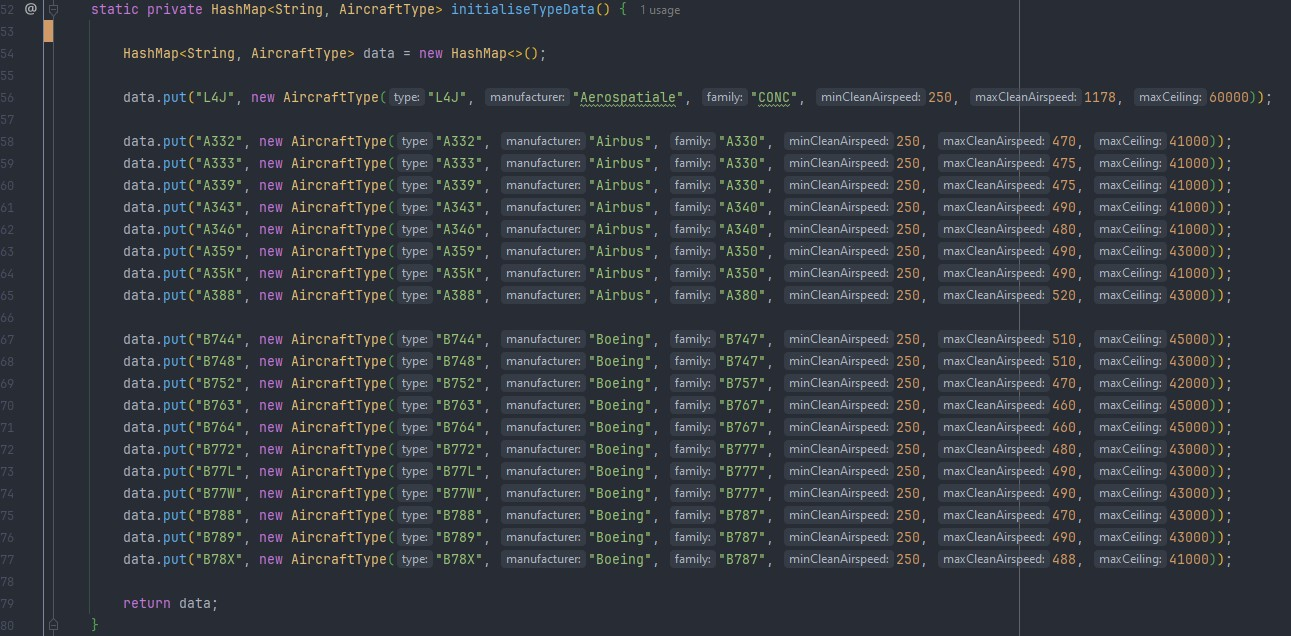
\includegraphics[width=1.1\textwidth]{pictures/Figure 2.8 FYP.jpg}    
\end{figure}

It is important to note that although the aircraft type “Concorde” is shown here, it was never used in the final simulation. Instead, it was a fallback aircraft, in the event that the software could not assign a valid aircraft type to a flight across the Atlantic, Concorde was assigned because it would give an obvious, detectable error, which is helpful, instead of the software crashing. This is very beneficial, as software crashes can be challenging and time-consuming to analyse.   

\subsection{Simulation Engine Development}
With all the data collated and created, the additional software development process can take place. Since the RADAR software was largely pre-existing, only a small amount of additional code had to be written, most of which was to do with creating air traffic in a specific way and then managing that traffic once it had been created. 

The simulation engine needs to handle aircraft in two distinct scenarios: the Organised Track System (OTS) and Zero Tracks. Additionally, the software needs to be easily configurable, with a simple setting to operate with, or without the organised tracks.

When aircraft cross the Atlantic without the OTS, they will fly directly between the Oceanic airspace’s entry/exit points. Due to a limitation in the RADAR software, they can only fly along a rhumb line, not great circles, so there is a slight inefficiency in the route they will plot.  

\subsubsection{Aircraft Creation Algorithm}
Since the simulations conducted only monitor aircraft over the North Atlantic Ocean, aircraft need to be created (spawned) at the start of the oceanic track and then despawned at the end. In terms of this simulation, the route/flight plan before and after these points is completely irrelevant. However, the aircraft’s departure and arrival aerodromes are used to decide which North Atlantic Track they use to cross the Atlantic when simulating with the Organised Track system.

Due to the complexity of a potential algorithm to match the latitude and longitude coordinates of a possible departure airport to the closest oceanic airspace entry point (same goes for destination and exit point) when using the zero track system, the arrival and destination airports are not computed inside the RADAR software. Instead, the zero track routes will be compared to the routes used during the use of the OTS. An approximation will be asserted, stating that a potential Atlantic crossing would be suitable for an aircraft operating between two airports.

In terms of actual traffic simulation, there are a few necessary features to ensure the final data is as realistic as possible:
\begin{enumerate}
    \item Traffic should not enter the oceanic airspace from the North American and European sides at the same time. Instead, traffic should mimic real-world operations by flying from North America to Europe between the hours of 1800 GMT and 0600 GMT, and fly from Europe to North America for the other 12 hours of the day. 
    \item Traffic should be intelligently created at the entry points of oceanic airspace, ensuring that all traffic spacing rules are enforced. This means that,
    \begin{enumerate}
        \item For OTS operations, traffic should be spaced by 60 nm of lateral separation,
        \item Traffic should be spaced by 20nm of lateral separation for zero track operations.
    \end{enumerate}
    \item There should not be a constant flow of traffic over the oceanic airspace, there should be some variation with the time of day.
\end{enumerate}

With each of the three requirements listed above, the aircraft creation algorithm was constructed.

The first requirement was met using a reasonably straightforward method. The RADAR engine’s internal clock system, called SkyTime was used to define several key sections of the simulation. For simplicity, it was decided that SkyTime 0 should represent midnight GMT and that the simulation would run for a total of 48 hours. Therefore, boundaries were set inside of the RADAR software’s SkyTime so that:

\begin{itemize}
    \item For the first 6 hours, the aircraft would fly from North America to Europe (00:00 - 06:00),
    \item For the next 12 hours, the aircraft would fly from Europe to North America (06:00 - 18:00),
    \item For the next 12 hours, the aircraft would fly from North America to Europe (18:00 - 30:00), 
    \item For the next 12 hours, the aircraft would fly from Europe ot North America (30:00 - 42:00),
    \item For the final 6 hours, the aircraft would fly from North America to Europe (42:00 - 48:00).
\end{itemize}

This represents the whole 48-hour simulation time. With this logic implemented, it is ensured that aircraft fly the correct routes at the correct time of day. 

It is important to note at this point that the internal SkyTime parameter is scalable. This means that at 60 times normal speed, a full 48 hours can be simulated in 48 minutes. At 600 times normal speed, 48 hours could be simulated within 4.8 minutes. Due to the software still being early in development (and therefore can be prone to small discrepancies), it was found that at anything beyond 100 times normal speed, the aircraft no longer behave properly. Therefore, all simulations were run at 60 times normal speed.

The second requirement is a piece of code that acts as an air traffic controller for the unsimulated airspace. The algorithm is very simple. When attempting to create an aircraft at an oceanic entry point, it first checks to see if another aircraft is already in range of the point it wishes to enter at; so in the case of OTS operations, less than 60 nm and in the case of zero track operations, 20 nm. 

Unfortunately, the code implementation of that was not as simple as it sounds, keeping track of potentially dozens of aircraft and the points they were just created at can be very resource-intensive on a system if not done properly. Therefore, great care had to be taken to make sure that aircraft were being stored in a sensible data structure, and then removed from it when they were further than the minimum separation distance from another aircraft behind them. This was achieved by tracking not in terms of aircraft, but in terms of the static entry points. Whenever an aircraft is created at an entry point, it checks to see if another aircraft is already in range. If not, the aircraft is successfully created. In the event that another aircraft is in range, the code computes the distance between the aircraft that was in range of the point, to see if it still is. If the aircraft is no longer in range of the point, it marks the point as clear next time an aircraft spawn is attempted. This method ensures that the resource-intensive distance check calculation is only computed when the simulation requires it.

Finally, to have traffic operate in a realistic manner (not a constant flow of traffic at all times of day), a normal distribution was used to spawn aircraft in the different phases, while also keeping in mind a total maximum number of aircraft that can operate over the 48-hour period. This maximum value will be tweaked and changed at a later date to see how both systems of air traffic management cope under different workloads. Each of the 5 phases in the bullet points above can be seen in Figure 2.9, each showing a clear bell-curve (normal distribution) for aircraft being created in the different phases of the simulation.      

\begin{figure}[H]
    \caption{This figure shows air traffic on the RADAR software's display. A clear normal distribution can be seen in the traffic density, with infrequent traffic at the start followed by a high density region of traffic in the middle and then a low density period at the end.}
    \label{fig:2.9}
    \centering
    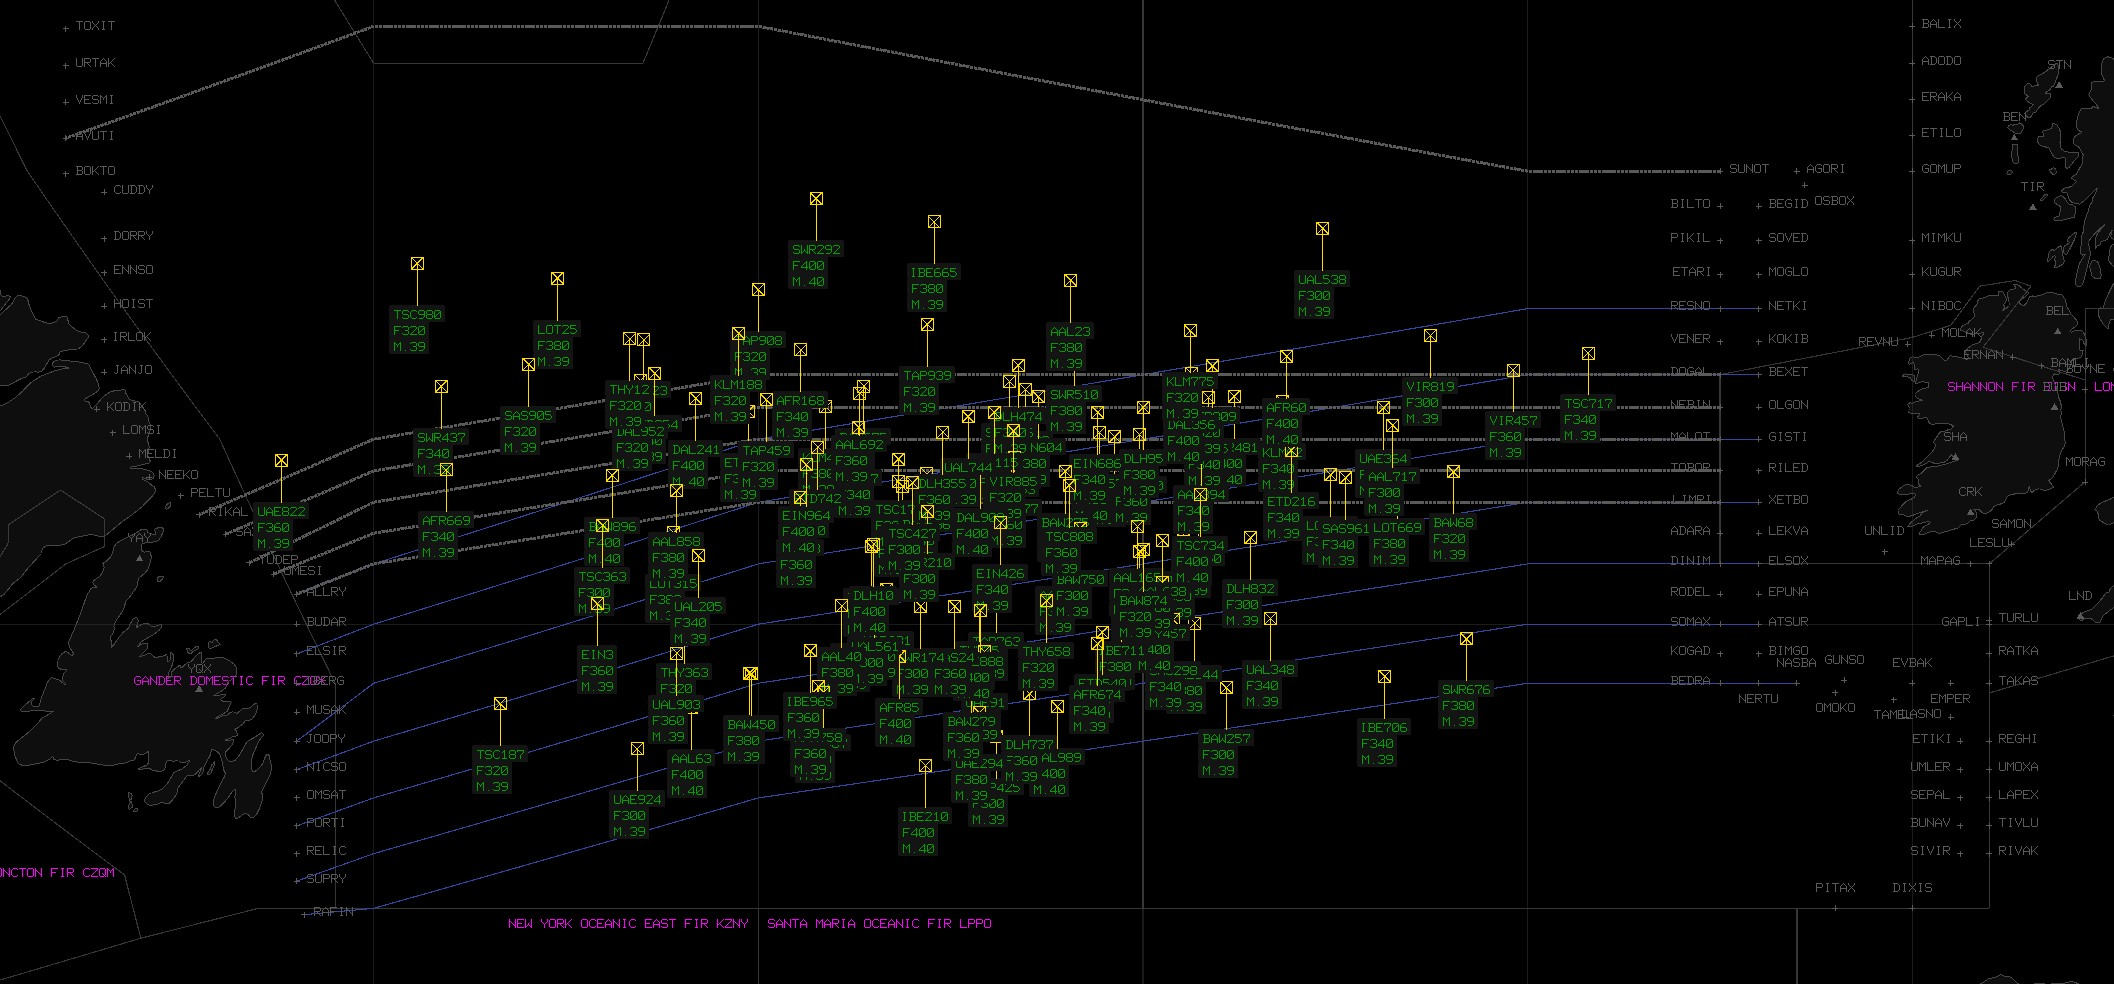
\includegraphics[width=1.1\textwidth]{pictures/Figure 2.9 FYP.jpg}    
\end{figure}

\subsubsection{Traffic Separation Algorithm}
As previously stated, in OTS operations and zero track operations, there are various minimum separation requirements which must be adhered to at all times. While the “air traffic controller” will ensure that no aircraft can be within the minimum separation distance when entering oceanic airspace, naturally, faster aircraft will catch up with slower flying ones. This poses a problem - do we make all aircraft slow down, or provide a capacity for aircraft to overtake one another? 

The latter option is most favourable for almost all circumstances, simply because different aircraft operate optimally at different speeds, therefore burning less fuel on their trans-Atlantic crossing. Therefore, when entering oceanic airspace, a separate process will take place, sorting aircraft’s altitude; slower aircraft fly lower, and therefore faster aircraft fly higher. For both OTS operations and zero track operations, minimum vertical separation is 1000ft, so increments of that value will be used to store aircraft. Furthermore, the semi-circular rule can be employed, so aircraft flying east will do so at an odd altitude, and aircraft flying west will do so at an even altitude. Figure 2.10 illustrates the semi-circular rule.  

Implementing this altitude-based separation system will solve most conflicts before aircraft get too close, especially for OTS operations. However, there also must be a system to monitor potential conflicts and take corrective action if needed; to do this, a primitive version of the Traffic Avoidance Collision System, or TCAS, was implemented into the RADAR software. In reality, TCAS is an emergency system that will take corrective action to avoid a mid-air collision between aircraft. It was chosen to mimic this functionality as ultimately any air traffic controller would have to take a similar course of action to prevent conflicts, whether using the OTS or zero tracks, the key difference is that TCAS activation in reality is a last-resort emergency action, when an air traffic controller should make such a corrective action in plenty of time. 

In terms of the RADAR software, each aircraft essentially operates with a bubble around it; in the event that different aircraft’s bubbles begin to intersect, they will take corrective action to avoid a collision. Importantly, the threshold for taking corrective action is highly configurable, so it can be modified to mimic keeping OTS separation requirements and zero track separation requirements. In addition, the RADAR software is capable of tracking the number of collisions per aircraft. Therefore, it can be studied which method of air traffic management requires more interventions for an air traffic controller. This will be one of the key parameters that are studied for the two methods of air traffic management.  
\subsection{Weather Simulation}
Weather remains an unpredictable element in aviation, even today, micro-bursts cause a significant danger to aircraft on final approaches. While weather is not as dangerous at thirty thousand feet and above (typical minimum altitude for trans-atlantic crossings) it can still have a major impact on aircraft efficiency. Headwinds can cause significant delays, while tailwinds can carry aircraft across the ocean much faster. In fact, each day the North Atlantic tracks are selected in part due to the weather prediction for that day, the goal is to provide aircraft with the best possible path over the ocean. However, there is still a significant degree of randomness when it comes to weather, take micro-bursts as a prime example. Simulating this randomness is non-trivial when it comes to computer software. 

When attempting to solve this problem, there were many different outcomes considered:
\begin{enumerate}
    \item A constant wind direction and speed throughout the whole simulation. This was ultimately not implemented due to the unrealistic nature of the weather being simulated. 
    \item Implement weather simulation based upon real world weather data published by the Met Office. This approach was considered and ultimately attempted, however it became apparent that it was simply too challenging and time consuming to implement into this project.
    \item Make no attempt to simulate the weather at all. Ultimately, this was the option selected. Simply but, this means the final simulation will not be flawless in terms of accuracy. However, it was decided that subjecting aircraft to all the same conditions (no weather) would provide a fairer result than subjecting aircraft in only one part of the sky to a weather condition at a constant rate, as described in the first bullet point. 
\end{enumerate}
The lack of weather simulation will be considered and discussed in relation to the final results, which will be discussed in Chapter 4. 
\subsection{Calibration}
The RADAR software is an experimental piece of equipment. While the level of confidence is high, there have been small bugs that have needed to be patched throughout the course of this project. Therefore, data produced by the software must be verified by real-world sources. This is another reason why real-world traffic data was analysed for this project. This means that each simulated aircraft can be compared with a real aircraft to make sure that the flight times are roughly similar, for the same flight types along the same route. Once this had been confirmed, the complete experimental testing process could begin. 
\subsection{Experimental Procedure}
Once the RADAR software was finalised and ready for testing, the experimental procedure was conducted. Several different traffic simulations were completed for both systems of air traffic management. The significant difference between the different simulations (other than method of air traffic management) was the number of aircraft simulated. In 2023, 580000 (\cite{ForeFlight}) aircraft made the crossing, so this means that approximately 1589 aircraft operated per day.

Therefore, the simulation was conducted for 1589 aircraft each day, for both OTS and zero tracks and then 10\% more and less than this value for both systems of air traffic management. From these simulations, the data relating to each aircraft will be collected, most importantly the simulated time for each aircraft as well as the number of correcting actions the aircraft experienced to maintain minimum separation. The results from these experiments will be found in the following chapter.

Each of these simulations will display information regarding how aircraft and the airspace itself performed in each scenario. The main metric that will be investigated for aircraft is their flight time to cross the Atlantic, whereas the main metric measured for the airspace is the total number of conflicts between aircraft; a conflict would require manual intervention by an air traffic controller. Remember, the simulation defines a conflict by an aircraft’s TCAS being activated and then avoiding action taking place to resolve the incident. In reality, TCAS is a system used in emergency situations only, not for traffic separation; therefore, the TCAS sensitivity was turned up, so it essentially functions as an air traffic controller, separating aircraft to ensure they comply with all regulations. 

Based on flight times for the aircraft flying between similar or the same destinations, a comment on fuel efficiency can be made (a shorter flight time means less fuel).

\newpage
\section{Results}
The results will be divided into six separate scenarios, each operating with different simulation parameters. The simulations conducted will show traffic for both the Organised Track System, and the zero track system of air traffic management at three levels of traffic density each: 100\% density, 1589 aircraft per day, 110\% density,  1748 aircraft per day and 90\% density, 1430 aircraft per day. Remember, each simulation lasts for 48 hours and therefore these numbers will be doubled. 

The actual number of aircraft simulated in each scenario may not be exactly equal to the number indicated; this is due to the normal distribution spawning pattern of aircraft having some variation. However, the number of aircraft spawned is no more than 10 different for each scenario. Each scenario was run at 60 times normal speed, so it took approximately 48 minutes to complete. 

Due to the fact that thousands of aircraft were simulated in each scenario, the full results will not be presented here, only a subsection. The full tables will be available in Appendix C.  
\subsection{Scenario 1: OTS System, 100\% Traffic Density}
The distribution of aircraft entering oceanic airspace for Scenario One can be seen below in Figure 3.1.
\begin{figure}[H]
    \caption{This figure shows the normal distribution of aircraft entering oceanic airspace in Scenario 1 over a 48 hour period.}
    \label{fig:3.1}
    \centering
    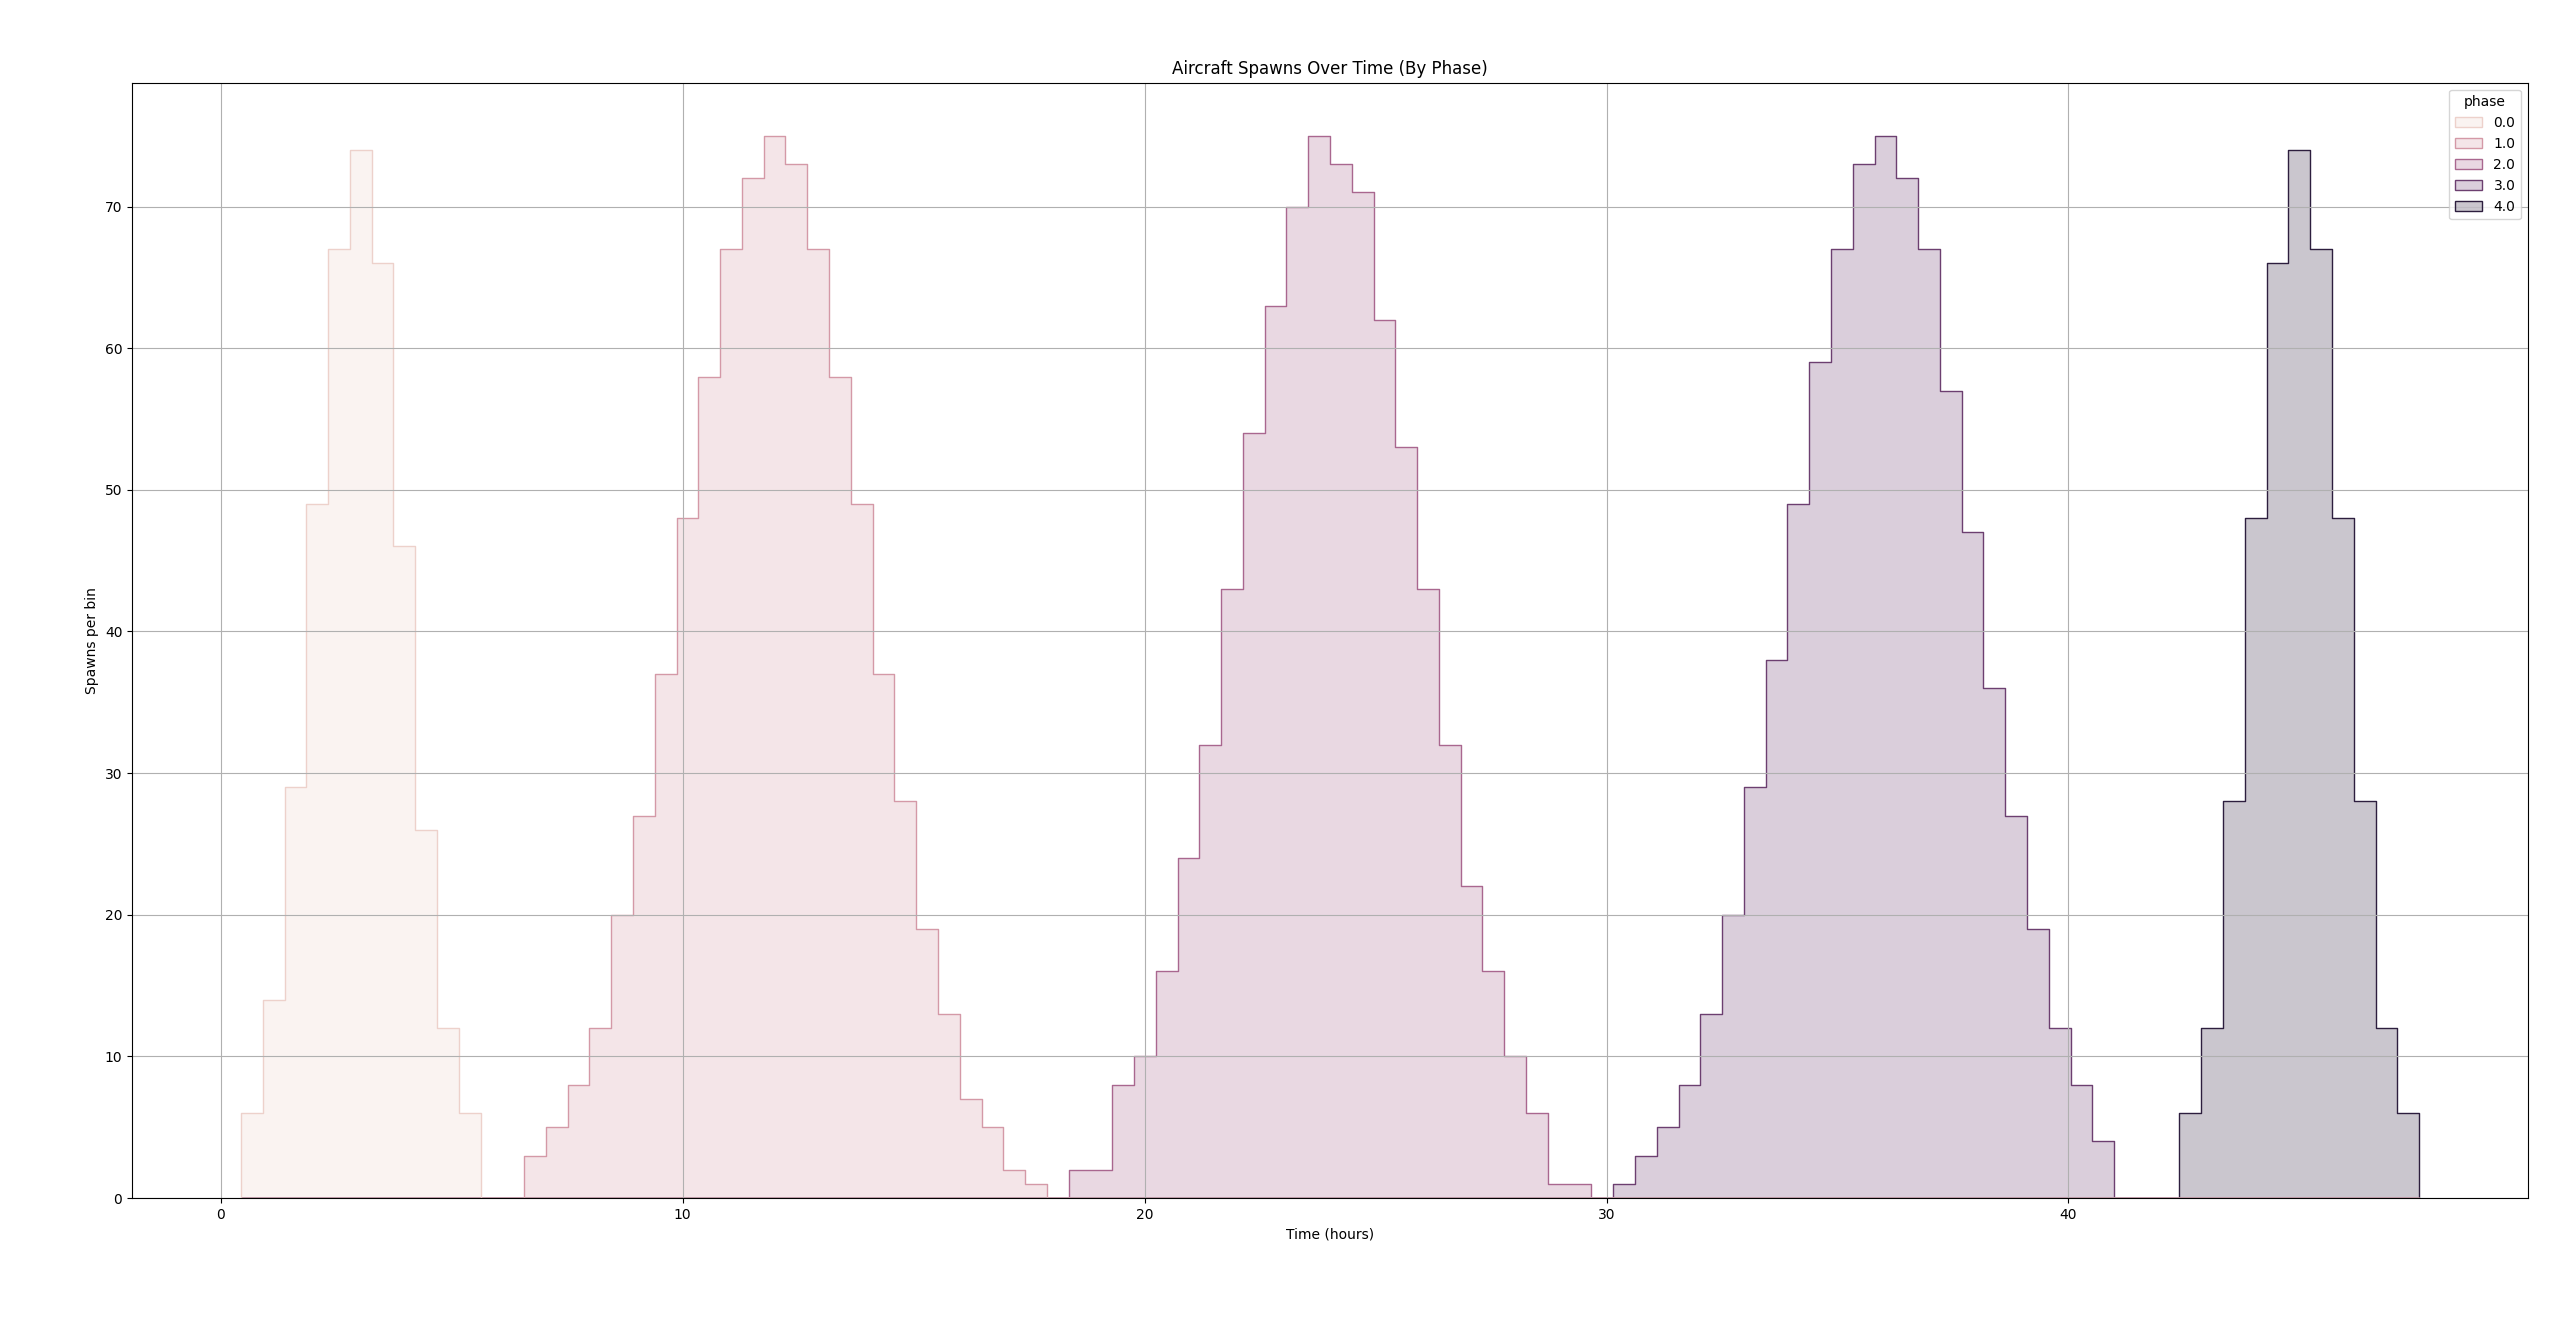
\includegraphics[width=1.1\textwidth]{pictures/Figure 3.1.png}    
\end{figure}
Figure 3.1 is useful as it provides clarification that the aircraft was created in a realistic and expected way by the software. It can easily be observed that the busiest time periods are in the middle of each oceanic crossing period. Furthermore, the first and final phases of the scenario have peaks that are much narrower; this is because their respective phases are cut short by the 48-hour simulation; they only last for 6 hours, whereas the others last for 48. We can expect to see a similar occurrence in the distribution of aircraft entering oceanic airspace in the other scenarios.
Table 3.1 shows the average information for the different types of air traffic that made the Atlantic crossing in this simulation. Throughout this 48-period, on 129 occasions, a traffic intervention occurred - preventing two aircraft from colliding. 

\begin{table}[H]
    \centering
    \caption{This table shows the simulation data for scenario one, for each of the different aircraft types that were included. The crossing time is given in minutes.}
    \label{tab:31}
    \begin{tabular}{@{}ccc@{}}
    \toprule
    \textbf{Aircraft Type} & \textbf{Number of Aircraft} & \textbf{Average Crossing Time} \\ \midrule
    B789                   & 277                         & 177.3                          \\
    B77W                   & 259                         & 176.3                          \\
    B788                   & 272                         & 185.2                          \\
    B772                   & 382                         & 181                            \\
    A359                   & 229                         & 177.4                          \\
    A333                   & 235                         & 183.4                          \\
    A332                   & 174                         & 183.9                          \\
    A339                   & 166                         & 182.3                          \\
    A35K                   & 132                         & 177.5                          \\
    B77L                   & 94                          & 175.9                          \\
    B748                   & 154                         & 169.7                          \\
    B78X                   & 111                         & 178.3                          \\
    B763                   & 212                         & 188.3                          \\
    B744                   & 139                         & 169.6                          \\
    B764                   & 102                         & 187.6                          \\
    A388                   & 105                         & 166.5                          \\
    A343                   & 25                          & 176.5                          \\
    B752                   & 38                          & 182.4                          \\
    A346                   & 53                          & 179.2                          \\ \bottomrule
    \end{tabular}
\end{table}
\subsection{Scenario 2: OTS System, 90\% Traffic Density}
The distribution of aircraft entering oceanic airspace for Scenario Two can be seen below in Figure 3.2.

\begin{figure}[H]
    \caption{This figure shows the normal distribution of aircraft entering oceanic airspace in Scenario 2 over a 48 hour period.}
    \label{fig:3.2}
    \centering
    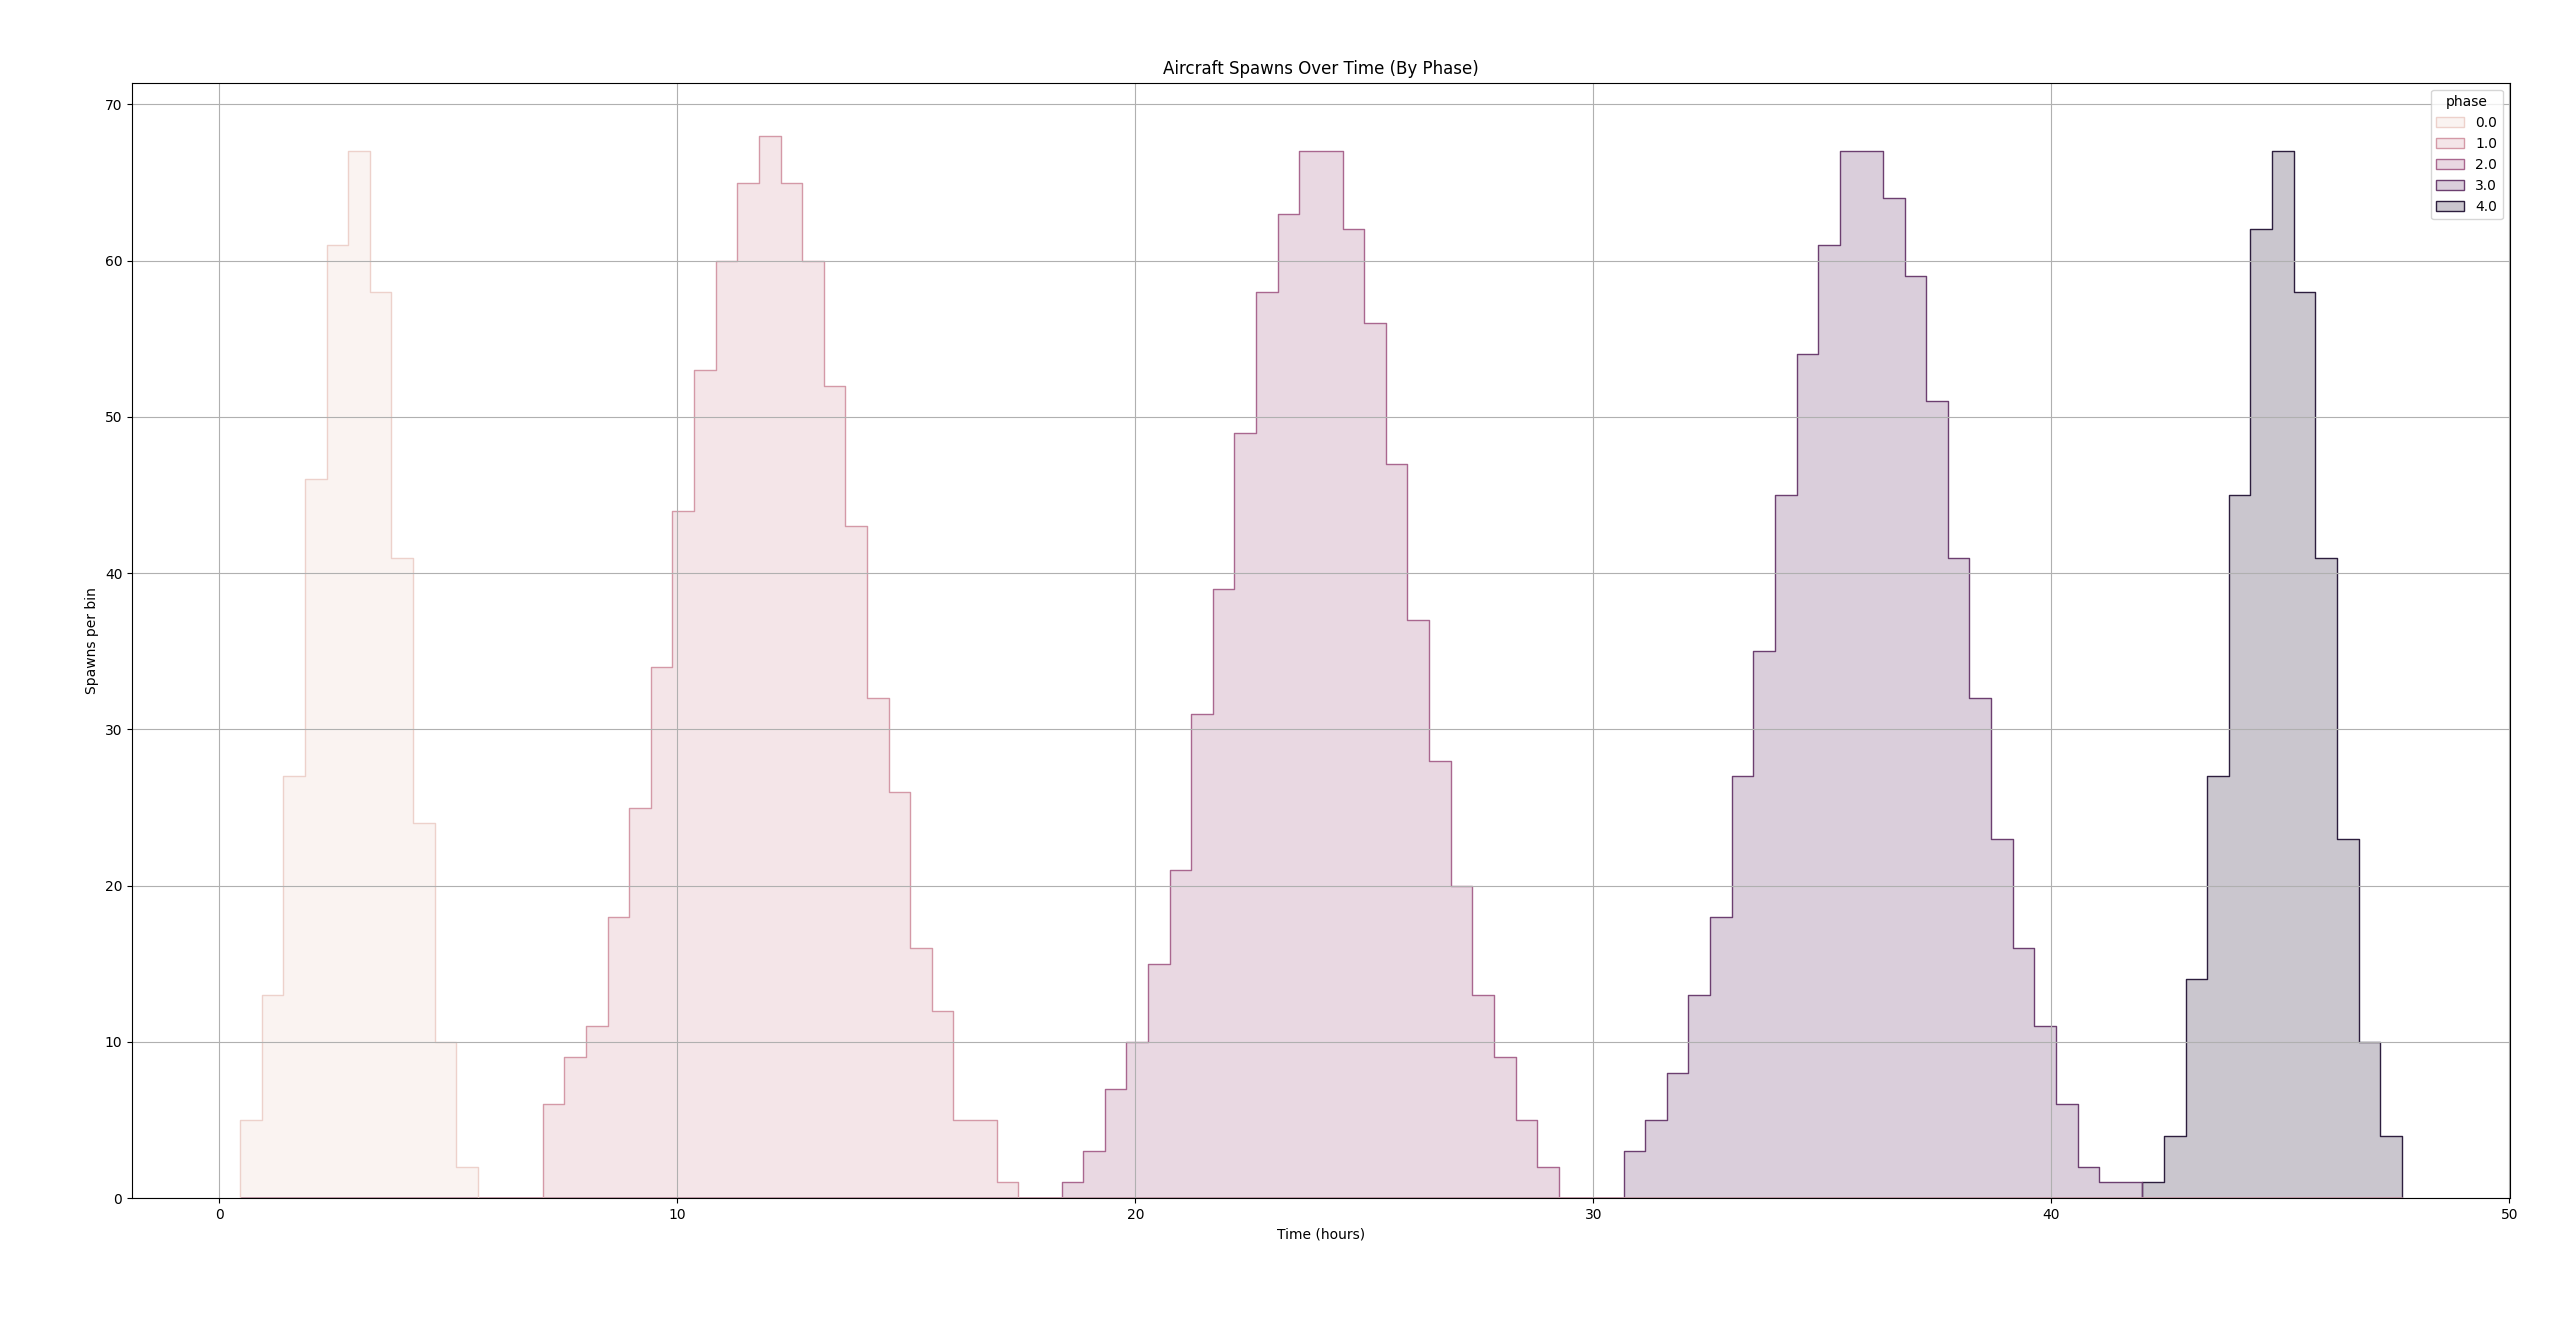
\includegraphics[width=1.1\textwidth]{pictures/Figure 3.2.png}    
\end{figure}

As expected, for Scenario Two, the peaks are lower than the distribution in Figure 3.1. This is another indication that the simulation was running as expected. 

Table 3.2 shows the average information for the different types of air traffic that made the Atlantic crossing in this simulation. Throughout this 48-period, on 124 occasions, a traffic intervention occurred - preventing two aircraft from colliding. The smaller number of conflicts is expected, as the amount of traffic operating has reduced by 10\%. However, the small difference observed between Scenarios One and Two suggests that there is not a proportional relationship between conflicts and the amount of air traffic.

\begin{table}[H]
    \centering
    \caption{This table shows the simulation data for scenario two, for each of the different aircraft types that were included. The crossing time is given in minutes.}
    \label{tab:32}
    \begin{tabular}{@{}ccc@{}}
    \toprule
    \textbf{Aircraft Type} & \textbf{Number of Aircraft} & \textbf{Average Crossing Time} \\ \midrule
    B789                   & 259                         & 177.3                          \\
    B77W                   & 240                         & 176.2                          \\
    B788                   & 245                         & 185.8                          \\
    B772                   & 340                         & 180.4                          \\
    A359                   & 194                         & 176.7                          \\
    A333                   & 217                         & 182                            \\
    A332                   & 166                         & 185.3                          \\
    A339                   & 135                         & 181.6                          \\
    A35K                   & 106                         & 177.3                          \\
    B77L                   & 96                          & 177.3                          \\
    B748                   & 130                         & 170.3                          \\
    B78X                   & 117                         & 176.7                          \\
    B763                   & 185                         & 188.7                          \\
    B744                   & 106                         & 169.6                          \\
    B764                   & 98                          & 189.3                          \\
    A388                   & 99                          & 166.9                          \\
    A343                   & 39                          & 175.7                          \\
    B752                   & 37                          & 183.4                          \\
    A346                   & 31                          & 179.4                          \\ \bottomrule
    \end{tabular}
\end{table}

\subsection{Scenario 3: OTS System, 110\% Traffic Density}
The distribution of aircraft entering oceanic airspace for Scenario Three can be seen below in Figure 3.3.

\begin{figure}[H]
    \caption{This figure shows the normal distribution of aircraft entering oceanic airspace in Scenario 3 over a 48 hour period.}
    \label{fig:3.3}
    \centering
    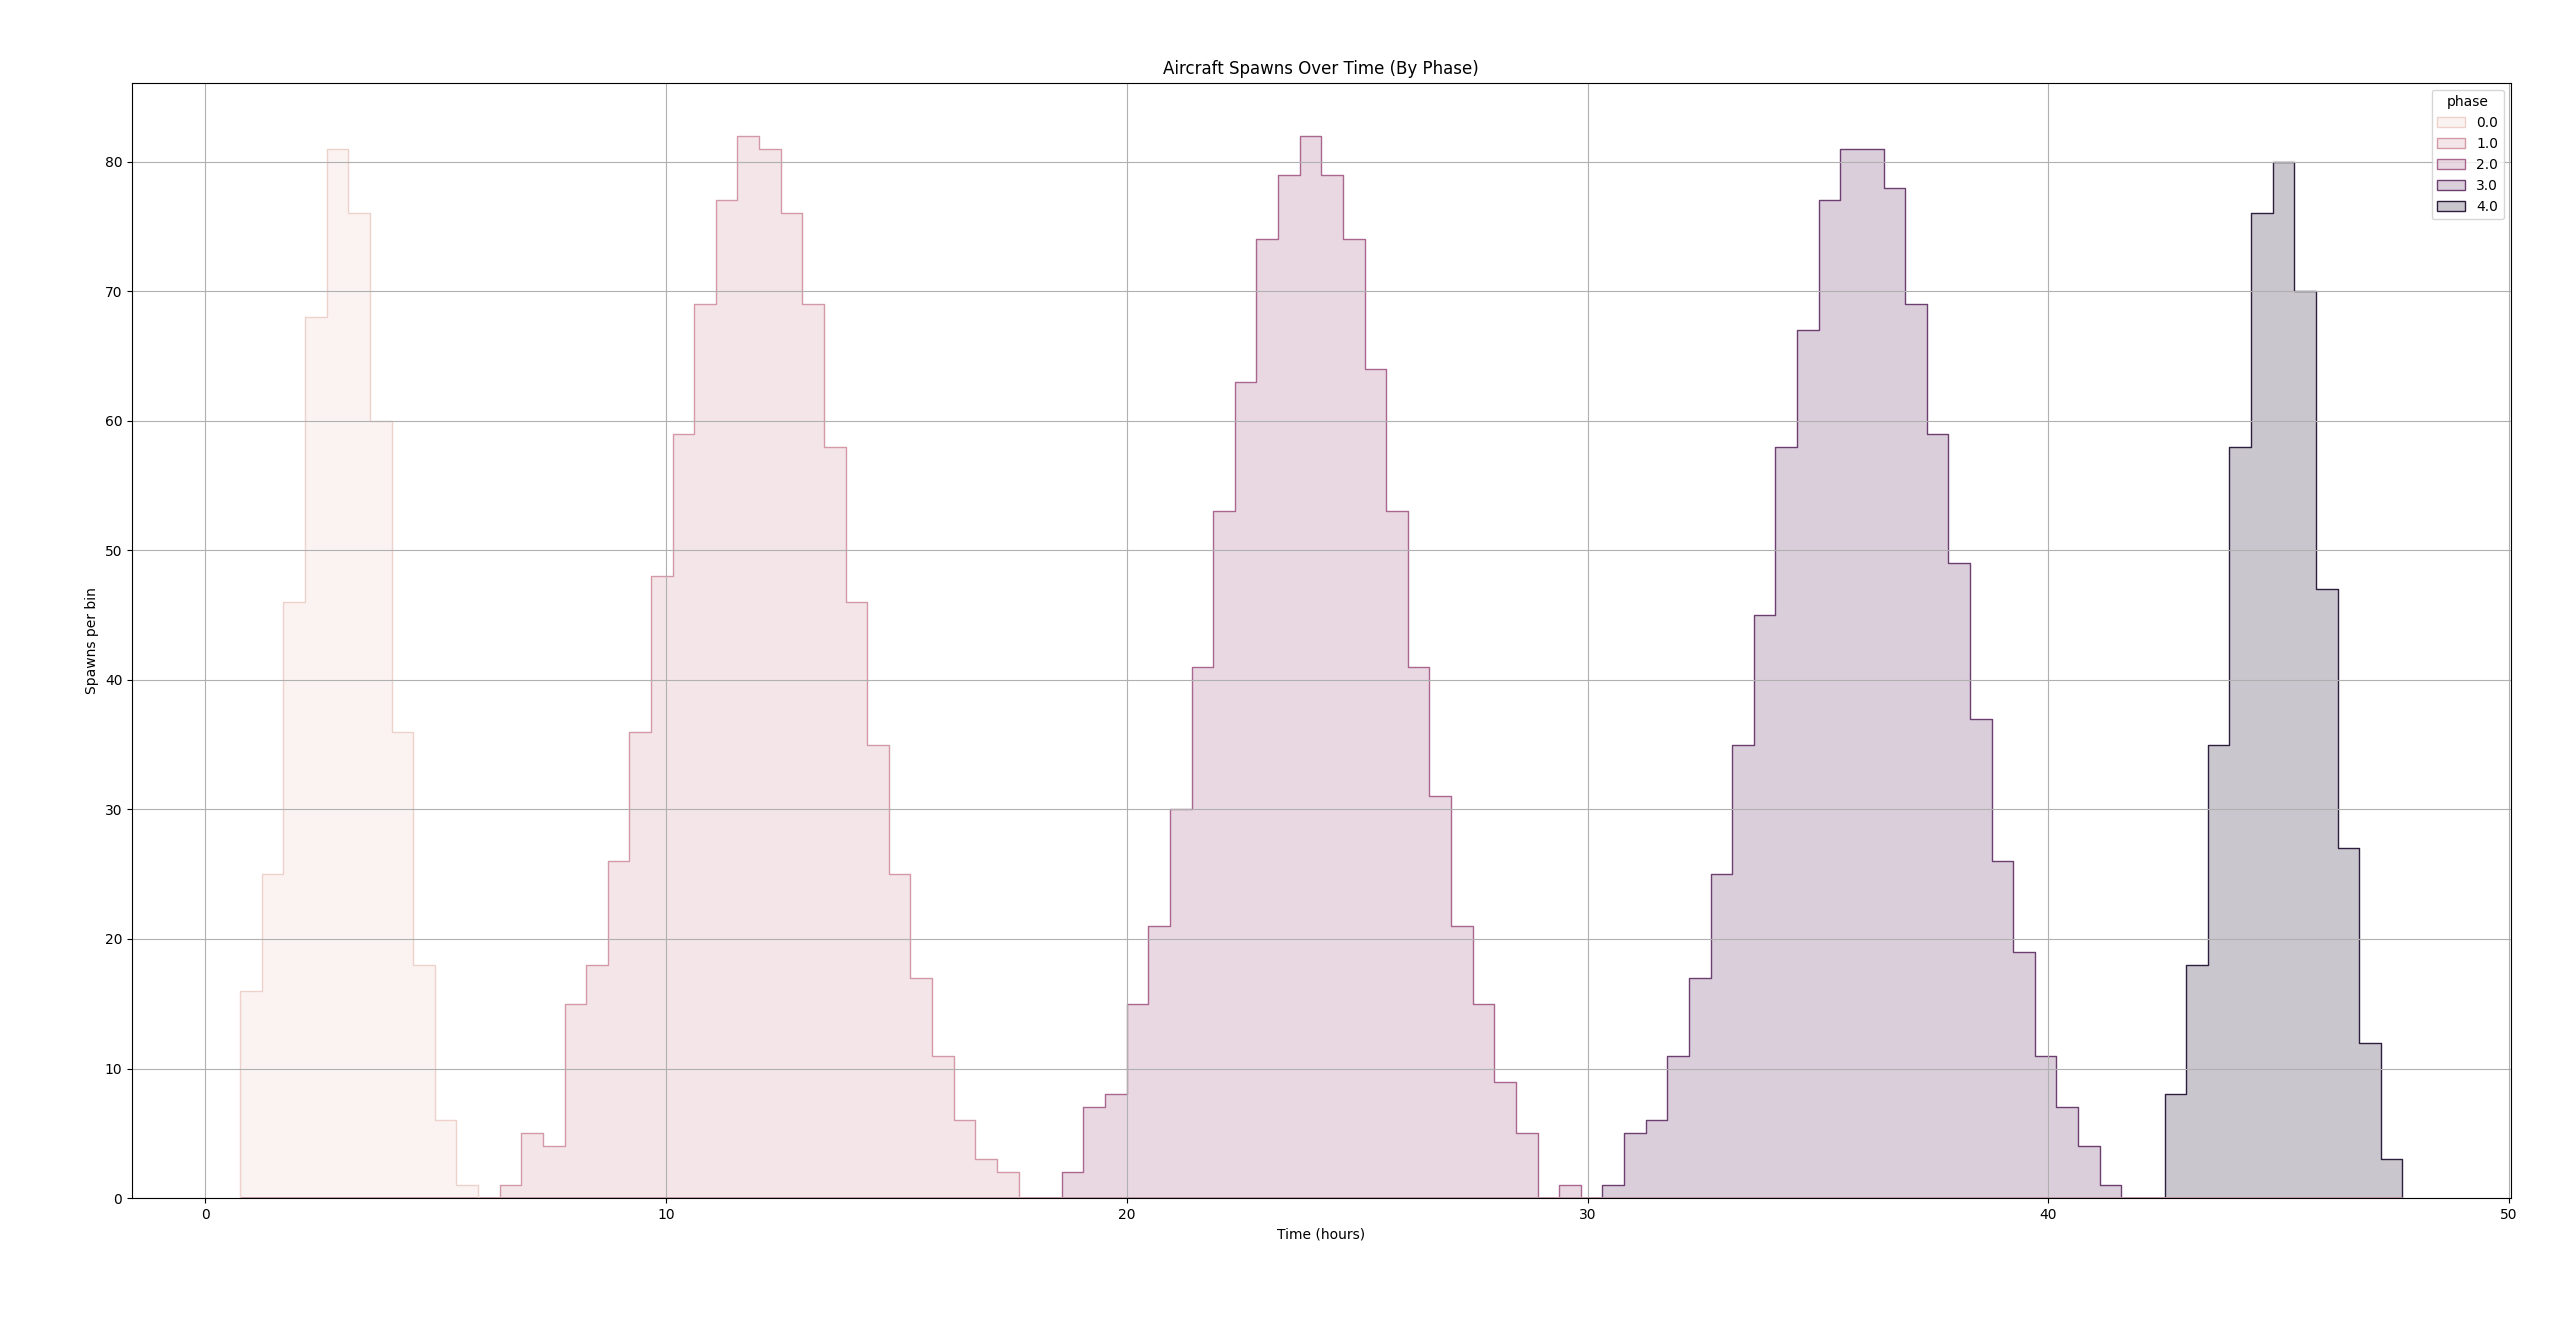
\includegraphics[width=1.1\textwidth]{pictures/Figure 3.3.png}    
\end{figure}

As expected, in Scenario Three, the peaks are much higher than those observed in Figures 3.1 and 3.2 as there is 10\% more traffic than normal operating on the Oceanic Tracks.

Table 3.3 shows the average information for the different types of air traffic that made the Atlantic crossing in this simulation. Throughout this 48 hour period, on 164 occasions, a traffic intervention occured - preventing two aircraft from colliding. This is a significantly higher number of interventions than those reported in Scenario 1, approximately 27\% more, again this suggests that there is a complex relationship between traffic density and the number of traffic interventions.

\begin{table}[H]
    \centering
    \caption{This table shows the simulation data for scenario three, for each of the different aircraft types that were included. The crossing time is given in minutes.}
    \label{tab:33}
    \begin{tabular}{@{}ccc@{}}
    \toprule
    \textbf{Aircraft Type} & \textbf{Number of Aircraft} & \textbf{Average Crossing Time} \\ \midrule
    B789                   & 329                         & 177                            \\
    B77W                   & 299                         & 177.2                          \\
    B788                   & 285                         & 184.3                          \\
    B772                   & 443                         & 180.4                          \\
    A359                   & 200                         & 176.9                          \\
    A333                   & 267                         & 182.4                          \\
    A332                   & 168                         & 184.6                          \\
    A339                   & 176                         & 182.8                          \\
    A35K                   & 128                         & 176.6                          \\
    B77L                   & 98                          & 178.3                          \\
    B748                   & 156                         & 169.8                          \\
    B78X                   & 125                         & 177.9                          \\
    B763                   & 245                         & 188.5                          \\
    B744                   & 158                         & 169.5                          \\
    B764                   & 149                         & 188.1                          \\
    A388                   & 152                         & 166.1                          \\
    A343                   & 23                          & 177.8                          \\
    B752                   & 26                          & 182.5                          \\
    A346                   & 46                          & 180.3                          \\ \bottomrule
    \end{tabular}
\end{table}
\subsection{Summary of Scenarios 1, 2 and 3}
Figure 3.4 shows the relationship between airspace density and number of aircraft interventions for the Organised Track System. This relationship appears to be exponential in nature, which ultimately makes sense considering the context, the more aircraft in a given piece of airspace, the higher the higher the likelihood is that it will conflict with something else. 
\begin{figure}[H]
    \caption{This graph shows the relationship between airspace density and number of aircraft interventions.}
    \label{fig:3.4}
    \centering
    \resizebox{1.0\textwidth}{!}{%
    \begin{tikzpicture}
        \begin{axis}[
            title={Rate of Increase of Aircraft Interventions with respect to Airspace Density for the OTS System},
            xlabel={\% Airspace Density},
            ylabel={Number of Interventions},
            xmin=85, xmax=115,
            ymin=120, ymax=170,
            xtick={90, 100, 110},
            ytick={120, 130, 140, 150, 160, 170},
            grid=both,
            width=14cm,
            height=8cm,
            thick
        ]
        \addplot[
            color=blue,
            mark=*,
            smooth
        ]
        coordinates {
            (90, 124)
            (100, 129)
            (110, 164)
        };
        \end{axis}
    \end{tikzpicture}
    }
\end{figure}
Additionally, Table 3.4 shows the percentage difference in the time it takes each aircraft type to fly over the Atlantic ocean, given the different airspace densities.
\begin{table}[H]
    \centering
    \caption{This table shows the percentage difference in Atlantic crossing times for the different aircraft types, when operating with the OTS at different airspace densities.}
    \label{tab:34}
    \begin{tabular}{@{}cc@{}}
    \toprule
    \textbf{Aircraft Type} & \textbf{Absolute Difference} \\ \midrule
    B789                   & 0.17\%                       \\
    B77W                   & 0.57\%                       \\
    B788                   & 0.81\%                       \\
    B772                   & 0.33\%                       \\
    A359                   & 0.40\%                       \\
    A333                   & 0.77\%                       \\
    A332                   & 0.76\%                       \\
    A339                   & 0.66\%                       \\
    A35K                   & 0.51\%                       \\
    B77L                   & 1.35\%                       \\
    B748                   & 0.35\%                       \\
    B78X                   & 0.90\%                       \\
    B763                   & 0.21\%                       \\
    B744                   & 0.06\%                       \\
    B764                   & 0.90\%                       \\
    A388                   & 0.48\%                       \\
    A343                   & 1.19\%                       \\
    B752                   & 0.55\%                       \\
    A346                   & 0.61\%                       \\ \bottomrule
    \end{tabular}
\end{table}

Ultimately, Table 3.4 shows that the airspace density has a very small to negligible impact on aircraft’s flight times across the Atlantic Ocean.

\subsection{Scenario 4: Zero Tracks System, 100\% Traffic Density}
The distribution of aircraft entering oceanic airspace for Scenario Four can be seen below in Figure 3.5.

\begin{figure}[H]
    \caption{This figure shows the normal distribution of aircraft entering oceanic airspace in Scenario 4 over a 48 hour period.}
    \label{fig:3.5}
    \centering
    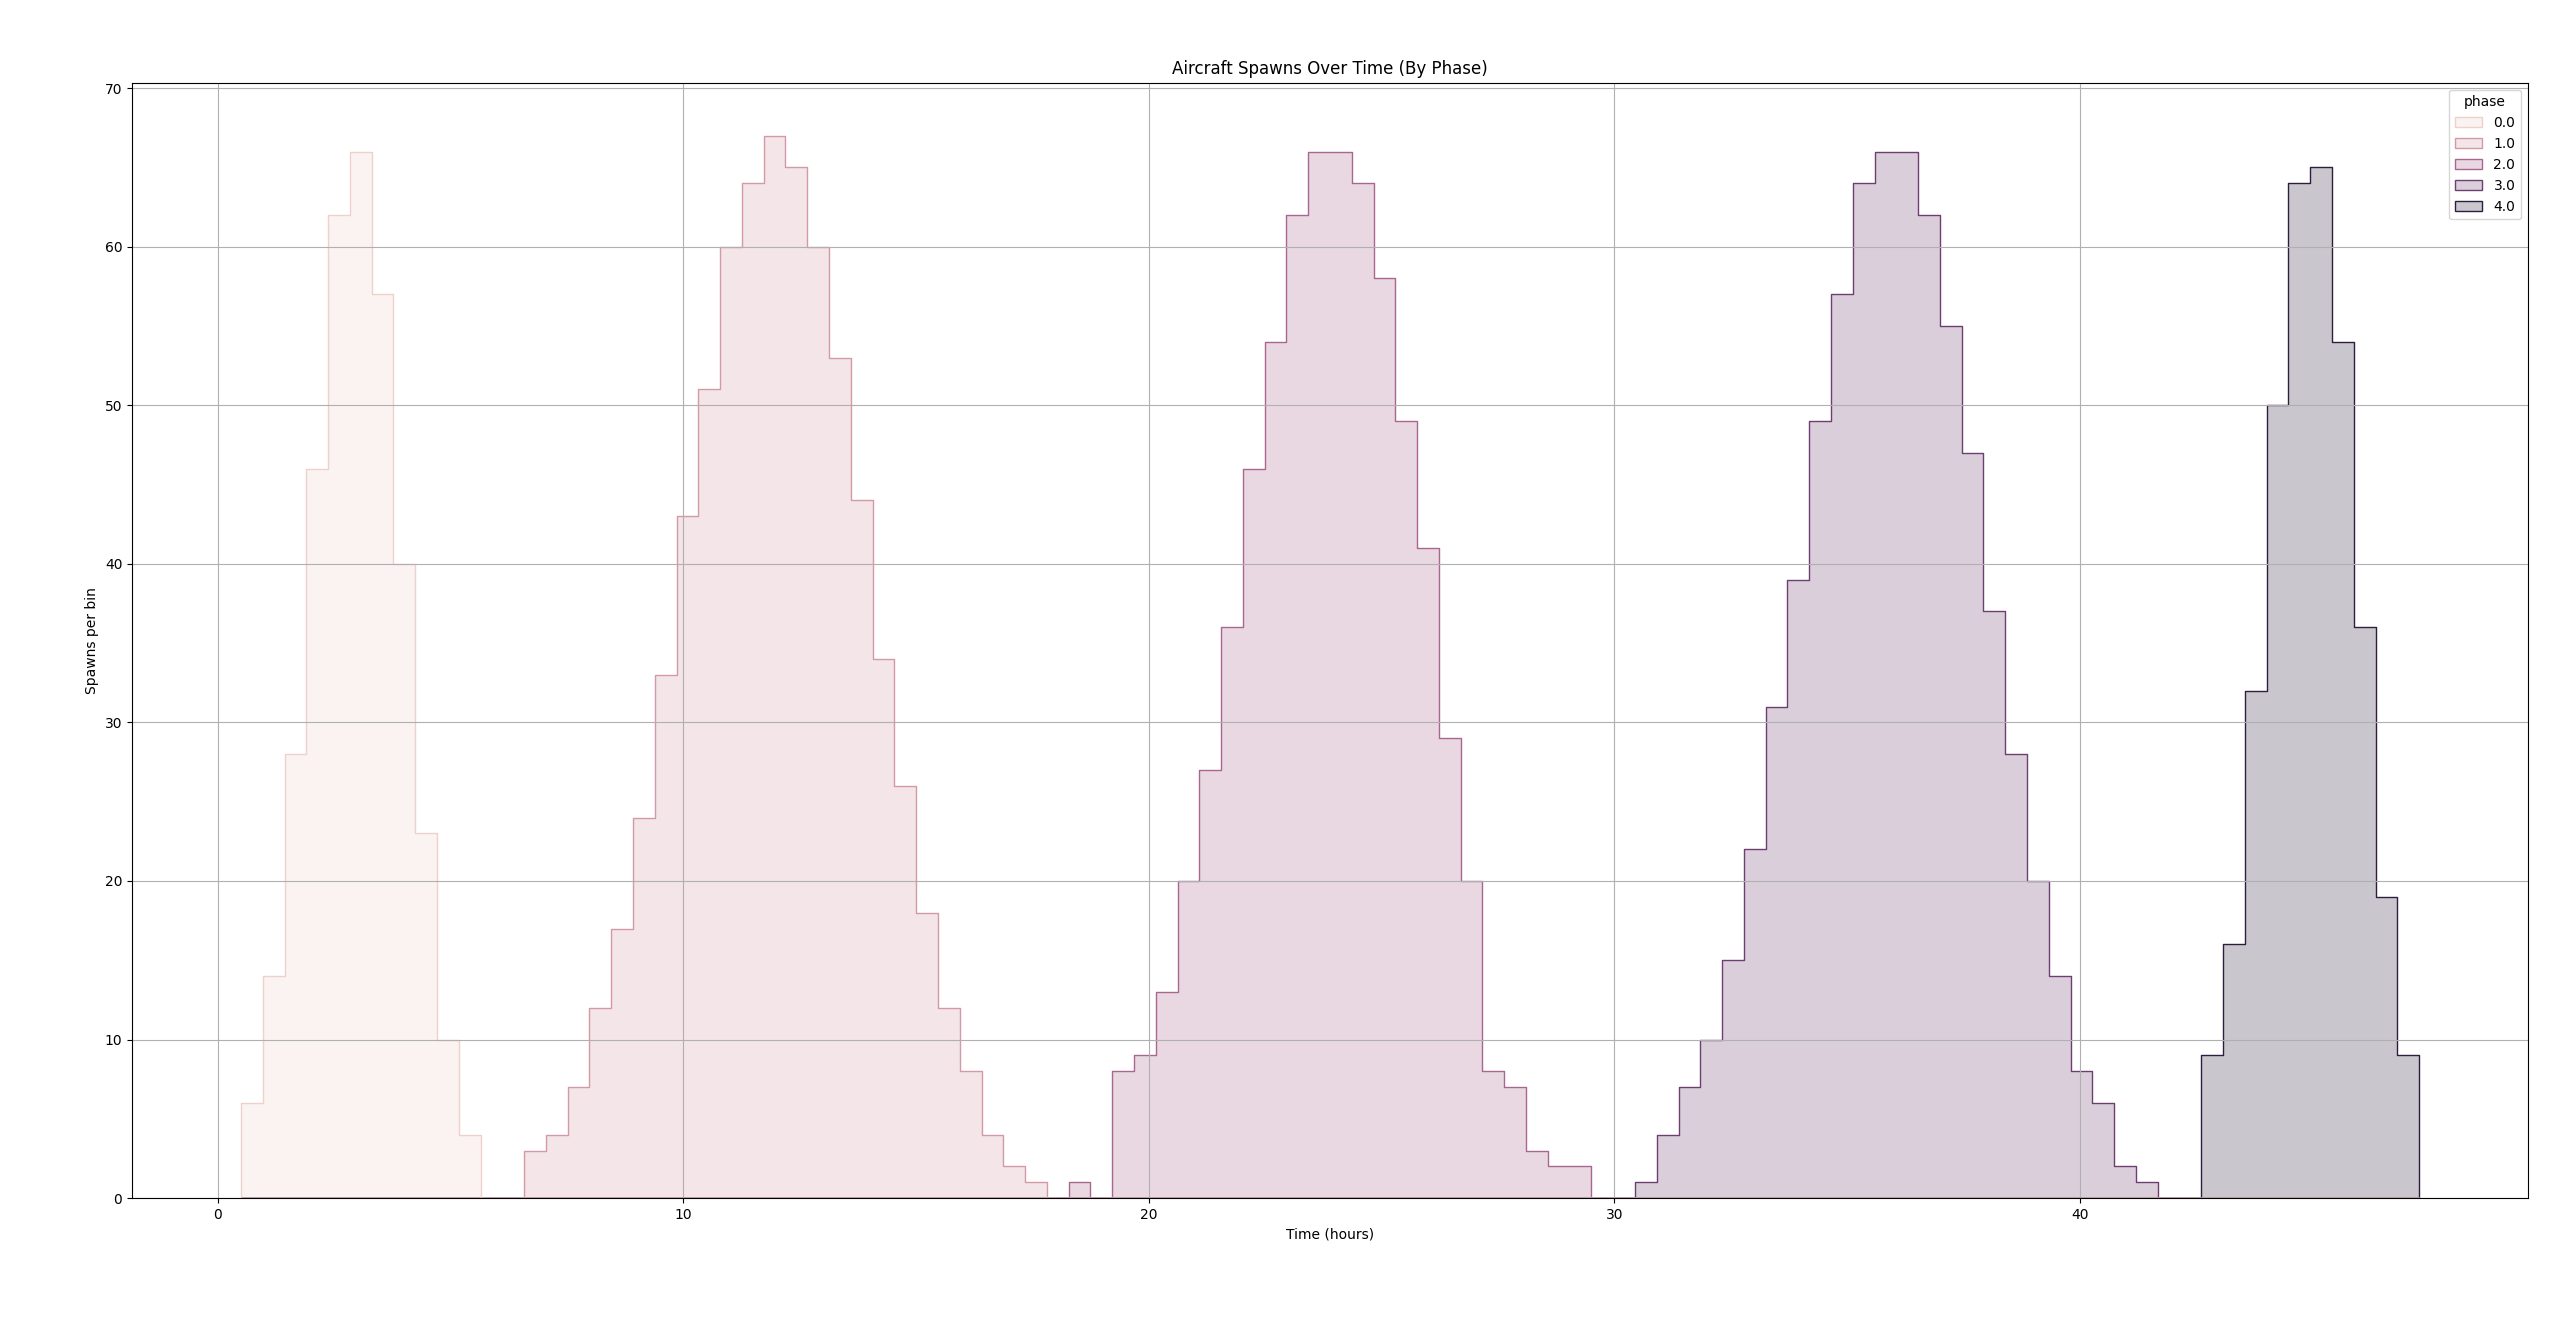
\includegraphics[width=1.1\textwidth]{pictures/Figure 3.5.png}    
\end{figure}

Table 3.5 shows the average information for the different types of air traffic that made the Atlantic crossing in this simulation. According to the software, on 118358 occasions throughout the 48-hour period, a traffic intervention occured - preventing two aircraft from colliding. This number is incredibly high and is likely incorrect due to several factors:
When visually inspecting the simulation (while in progress), there are not this many conflicts. 
If true, there would be a conflict roughly every two seconds (assuming a constant stream of traffic, which we know is not the case). 
Unfortunately, very late into the project, a “bug” inside of the RADAR software was encountered, which triggered the logging of a conflict numerous times per conflict. The effect of this bug got exponentially larger as the number of conflicts increased.

\begin{table}[H]
    \centering
    \caption{This table shows the simulation data for scenario four, for each of the different aircraft types that were included. The crossing time is given in minutes.}
    \label{tab:3.5}
    \begin{tabular}{@{}ccc@{}}
    \toprule
    \textbf{Aircraft Type} & \textbf{Number of Aircraft} & \textbf{Average Crossing Time} \\ \midrule
    B789                   & 372                         & 141.6                          \\
    B77W                   & 319                         & 147.6                          \\
    B788                   & 320                         & 150.6                          \\
    B772                   & 316                         & 158.2                          \\
    A359                   & 273                         & 141.7                          \\
    A333                   & 242                         & 144.9                          \\
    A332                   & 206                         & 149.7                          \\
    A339                   & 178                         & 156.1                          \\
    A35K                   & 141                         & 132.6                          \\
    B77L                   & 127                         & 143                            \\
    B748                   & 98                          & 158.5                          \\
    B78X                   & 92                          & 159.8                          \\
    B763                   & 131                         & 177.7                          \\
    B744                   & 96                          & 161.5                          \\
    B764                   & 68                          & 178.6                          \\
    A388                   & 81                          & 148.3                          \\
    A343                   & 27                          & 142.9                          \\
    B752                   & 29                          & 171.2                          \\
    A346                   & 41                          & 137.8                          \\ \bottomrule
    \end{tabular}
\end{table}

\subsection{Scenario 5: Zero Tracks System, 90\% Traffic Density}
The distribution of aircraft entering oceanic airspace for Scenario Five can be seen below in Figure 3.6.

\begin{figure}[H]
    \caption{This figure shows the normal distribution of aircraft entering oceanic airspace in Scenario 5 over a 48 hour period.}
    \label{fig:3.6}
    \centering
    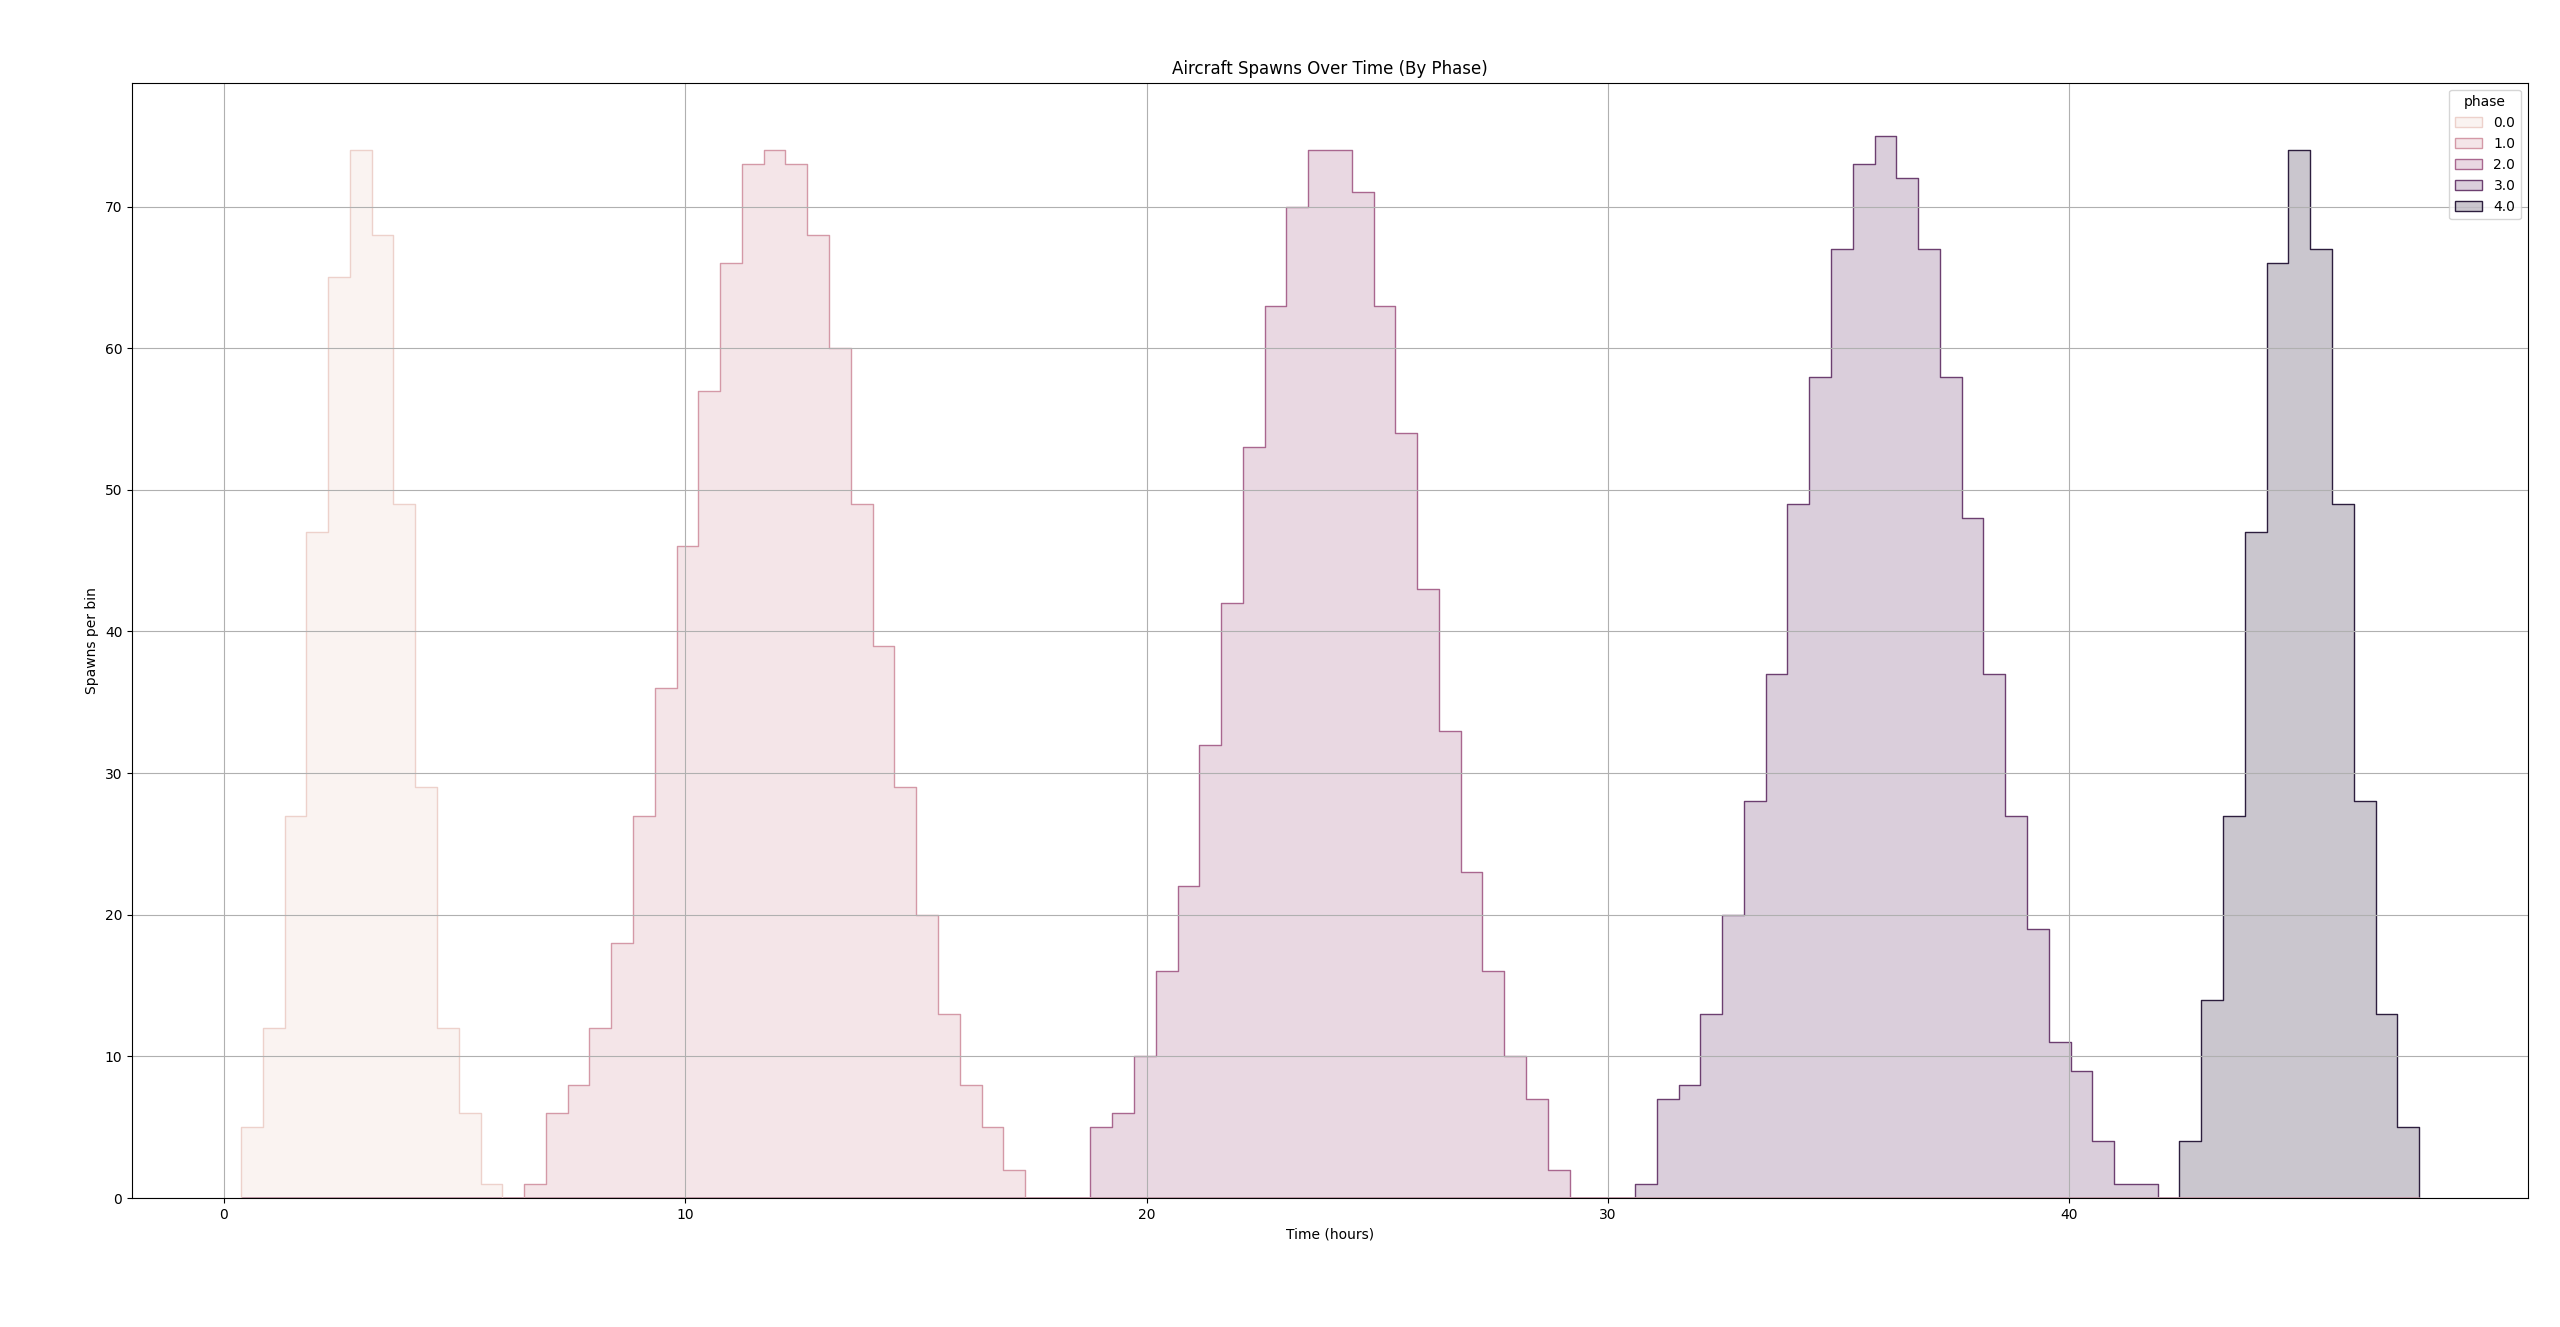
\includegraphics[width=1.1\textwidth]{pictures/Figure 3.6.png}    
\end{figure}

Table 3.6 shows the average information for the different types of air traffic that made the Atlantic crossing in this simulation. According to the software, on 60719 occasions throughout the 48-hour period, a traffic intervention occured - preventing two aircraft from colliding. Clearly, the “bug” discussed in Scenario 4 is still present here. However, the difference can be observed to be significantly smaller. From this it can be inferred that for the zero track system, traffic density has a much larger impact on conflicts compared to the OTS. 

\begin{table}[H]
    \centering
    \caption{This table shows the simulation data for scenario five, for each of the different aircraft types that were included. The crossing time is given in minutes.}
    \label{tab:36}
    \begin{tabular}{@{}ccc@{}}
    \toprule
    \textbf{Aircraft Type} & \textbf{Number of Aircraft} & \textbf{Average Crossing Time} \\ \midrule
    B789                   & 267                         & 135.5                          \\
    B77W                   & 247                         & 128.3                          \\
    B788                   & 231                         & 133.6                          \\
    B772                   & 229                         & 164.4                          \\
    A359                   & 174                         & 129.7                          \\
    A333                   & 185                         & 139.5                          \\
    A332                   & 137                         & 142                            \\
    A339                   & 132                         & 142.3                          \\
    A35K                   & 106                         & 144.5                          \\
    B77L                   & 78                          & 134.5                          \\
    B748                   & 72                          & 160.1                          \\
    B78X                   & 66                          & 154.1                          \\
    B763                   & 108                         & 182.1                          \\
    B744                   & 79                          & 156.2                          \\
    B764                   & 53                          & 180.9                          \\
    A388                   & 45                          & 159.4                          \\
    A343                   & 26                          & 141.6                          \\
    B752                   & 19                          & 152                            \\
    A346                   & 23                          & 165.6                          \\ \bottomrule
    \end{tabular}
\end{table}

\subsection{Scenario 6: Zero Tracks System, 110\% Traffic Density}
The distribution of aircraft entering oceanic airspace for Scenario Five can be seen below in Figure 3.7.

\begin{figure}[H]
    \caption{This figure shows the normal distribution of aircraft entering oceanic airspace in Scenario 6 over a 48 hour period.}
    \label{fig:3.7}
    \centering
    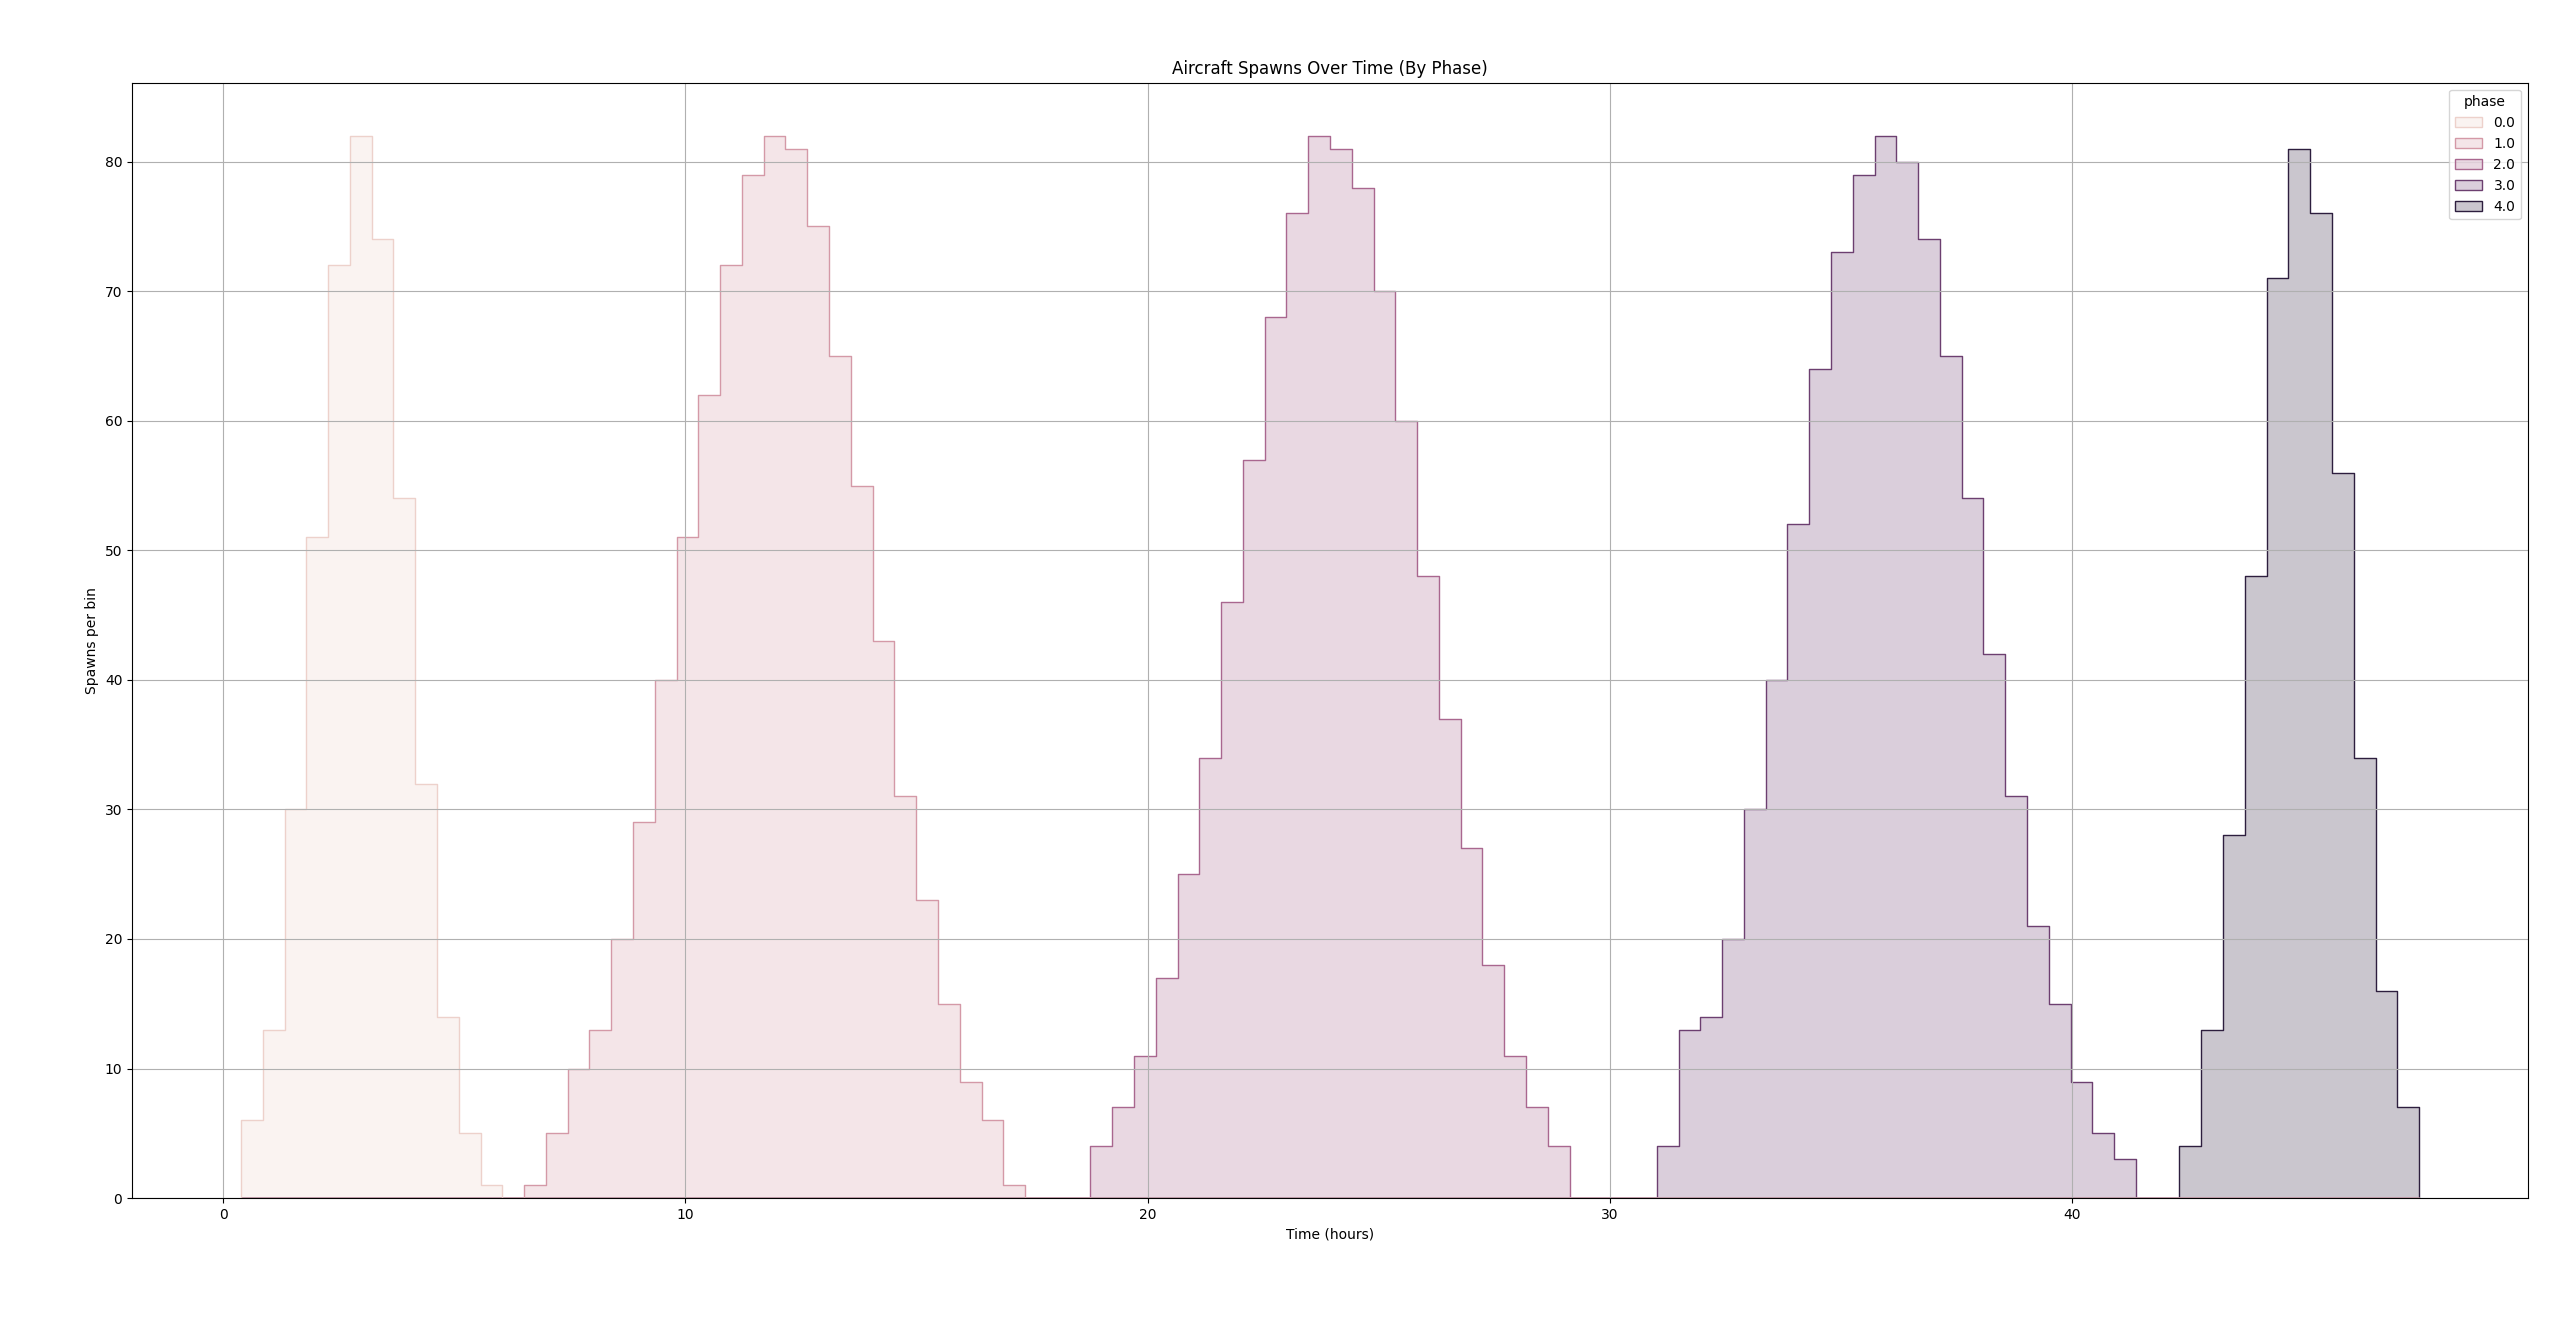
\includegraphics[width=1.1\textwidth]{pictures/Figure 3.7.png}    
\end{figure}

Table 3.7 shows the average information for the different types of air traffic that made the Atlantic crossing in this simulation. According to the software, on 177004 occasions throughout the 48-hour period, a traffic intervention occured - preventing two aircraft from colliding. The same issue is clearly present again. However, it should be noted that the difference between the value observed in Scenario 4 could still be useful.

\begin{table}[H]
    \centering
    \caption{This table shows the simulation data for scenario six, for each of the different aircraft types that were included. The crossing time is given in minutes.}
    \label{tab:37}
    \begin{tabular}{@{}ccc@{}}
    \toprule
    \textbf{Aircraft Type} & \textbf{Number of Aircraft} & \textbf{Average Crossing Time} \\ \midrule
    B789                   & 426                         & 140.1                          \\
    B77W                   & 359                         & 140.8                          \\
    B788                   & 311                         & 154.6                          \\
    B772                   & 360                         & 156.9                          \\
    A359                   & 274                         & 136.9                          \\
    A333                   & 307                         & 150                            \\
    A332                   & 168                         & 148.3                          \\
    A339                   & 199                         & 137.7                          \\
    A35K                   & 169                         & 143.4                          \\
    B77L                   & 141                         & 142.6                          \\
    B748                   & 107                         & 158                            \\
    B78X                   & 113                         & 155.5                          \\
    B763                   & 154                         & 174.8                          \\
    B744                   & 102                         & 152.3                          \\
    B764                   & 82                          & 170.5                          \\
    A388                   & 85                          & 151.6                          \\
    A343                   & 42                          & 127.7                          \\
    B752                   & 33                          & 149.5                          \\
    A346                   & 42                          & 156.8                          \\ \bottomrule
    \end{tabular}
\end{table}
\subsection{Summary of Scenarios 4, 5 and 6}
Figure 3.8 shows the relationship between airspace density and number of aircraft interventions for the Zero Track System. This relationship appears to be linear in nature. However, it must be remembered that the values obtained are clearly incorrect due to the bug in the RADAR software. The linear relationship, however, is useful to be aware of.

\begin{figure}[H]
    \caption{This graph shows the relationship between airspace density and number of aircraft interventions.}
    \label{fig:3.4}
    \centering
    \resizebox{1.0\textwidth}{!}{%
    \begin{tikzpicture}
        \begin{axis}[
            title={Rate of Increase of Aircraft Interventions with respect to Airspace Density for the OTS System},
            xlabel={\% Airspace Density},
            ylabel={Number of Interventions},
            xmin=85, xmax=115,
            ymin=60000, ymax=180000,
            xtick={90, 100, 110},
            ytick={60000, 80000, 100000, 120000, 140000, 160000, 180000},
            grid=both,
            width=14cm,
            height=8cm,
            thick
        ]
        \addplot[
            color=blue,
            mark=*,
            smooth
        ]
        coordinates {
            (90, 60719)
            (100, 118358)
            (110, 177004)
        };
        \end{axis}
    \end{tikzpicture}
    }
\end{figure}

Additionally, Table 3.8 shows the percentage difference in the time it takes each aircraft type to fly over the Atlantic Ocean, given the different airspace densities.

\begin{table}[H]
    \centering
    \caption{This table shows the percentage difference in Atlantic crossing times for the different aircraft types, when operating with the Zero Track System at different airspace densities.}
    \label{tab:38}
    \begin{tabular}{@{}cc@{}}
    \toprule
    \textbf{Aircraft Type} & \textbf{Absolute Difference} \\ \midrule
    B789                   & 4.39\%                       \\
    B77W                   & 13.89\%                      \\
    B788                   & 14.36\%                      \\
    B772                   & 4.69\%                       \\
    A359                   & 8.82\%                       \\
    A333                   & 7.25\%                       \\
    A332                   & 5.25\%                       \\
    A339                   & 12.66\%                      \\
    A35K                   & 8.49\%                       \\
    B77L                   & 6.07\%                       \\
    B748                   & 1.32\%                       \\
    B78X                   & 3.64\%                       \\
    B763                   & 4.10\%                       \\
    B744                   & 5.87\%                       \\
    B764                   & 5.89\%                       \\
    A388                   & 7.25\%                       \\
    A343                   & 11.06\%                      \\
    B752                   & 13.77\%                      \\
    A346                   & 18.12\%                      \\ \bottomrule
    \end{tabular}
\end{table}

Ultimately, Table 3.8 shows that the airspace density has a somewhat significant impact on the time it takes to cross the Atlantic, with the highest difference being 18.12\%.  

\subsection{Overall Summary of Results}
Ultimately, there are several key observations that can be taken away from the simulations:
\begin{enumerate}
    \item The time taken for aircraft to cross the North Atlantic Ocean is much smaller using the Zero Track system compared to the OTS. 
    \item Traffic Density has a much bigger impact on flight times for the Zero Track system compared to the OTS. 
    \item The relationship of interventions to traffic density is exponential for the OTS, but linear for the Zero Track System (although there is a flaw with the software that could have manipulated this relationship). 
\end{enumerate}

\newpage
\section{Discussion}
Assessing the two different methods of air traffic management is not an easy task, both systems clearly have positives and negatives. 

First of all, the OTS is limited by its own design; there can only be so many aircraft on each oceanic track at any given moment in time due to the strict separation requirements. Additionally, the OTS does not tend to follow the most direct path across the Atlantic, in Tables 3.1 and 3.4 (100\% traffic density for OTS and zero tracks, respectively), time differences between 20 and 30 minutes for most aircraft can be observed. This is not an insignificant amount of time, both in terms of the environmental impact of burning aviation fuel, but also in terms of extra time that is freed up in the aircraft’s schedule. The longer a flight takes, the more fuel it requires. Not only does this extra fuel come at a cost to the environment, but it also impacts those who wish to travel by aircraft; more fuel means an increased ticket price. This is why low-cost airlines charge so much for extra baggage and are so strict on the maximum suitcase dimensions and weight. Making travel by aviation cheaper, and therefore more accessible, will only result in positives for the industry; more customers mean more streams of revenue. For the airlines, shorter flights mean that there is the potential for longer turnaround times at major airports (assuming the airport has capacity for such a thing). More importantly, it adds extra slack in a very tight schedule. If a long turnaround is planned, it means that there is a bigger opportunity to make up time in the event of delays. 

However, the Zero track system is also limited as it requires a more “hands on approach” by air traffic controllers. Even though the raw data provided by the simulation is clearly wrong, it is clear that there is a higher number of traffic conflicts when using the zero track system. This assertion can be made because of the nature of the bug, which was previously explained. The more conflicts that are detected, the more out of sync the RADAR software gets, logging the same conflicts an increasing number of times each. However, this is hardly surprising. Aircraft operating between any entry and exit point in oceanic airspace is bound to result in aircraft flying over eachother’s paths, resulting in conflicts. 

In addition, the simulation produced in the RADAR software is purely reactionary in nature in its approach to dealing with conflicts in the sense that if a problem comes up, it will deal with it then. A better approach would be to plan aircraft in a sequence that minimises potential route crossings. This simply could not be simulated for this project due to the intense processing power required for such a calculation; it was simply not possible inside the software used. However, it would be very achievable for two large governmental organisations such as NAV Canada and NATS. 

The lack of weather simulation cannot be ignored. In reality, the Oceanic Tracks are picked partially to make use of the weather, giving aircraft the most optimum route, usually involving a large tailwind component. That, of course, has not been considered in this simulation, nor has the effect of any potential headwind. This is not an insignificant factor, as some zero track paths may end up taking longer to complete than the North Atlantic Tracks because of the headwind component. Additionally, the aircraft in the RADAR simulation fly along rhumb lines when not following a NAT track; in reality, they would be more likely to follow a great circle, as they are always the shortest possible distance. These two factors combined may result in the Oceanic crossing time for the zero track system to increase, but it is not possible to reasonably quantify how big this impact is. 

Outside of the Aircraft Surveillance scope, the introduction of Space-Based ADS-B technology has resulted in the ability to track aircraft anywhere on the globe. This has major implications, mostly in the event of catastrophic failure. Take Malaysian Airlines Flight 370, for example, an aircraft that vanished while operating in a “RADAR dead” part of south-east Asia. With the introduction of Aircraft Tracking, thanks to Space-Based ADS-B technology provided by Aireon, aircraft can be monitored anywhere on the globe. While this will not prevent accidents, like the kind that happened to MH 370, they will aid in the subsequent investigation and therefore provide information that can be learned from going forward.

\newpage
\section{Conclusions}
\section{Recommendations}

\printbibliography

\end{document}